\documentclass{article}\usepackage[]{graphicx}\usepackage[]{color}
%% maxwidth is the original width if it is less than linewidth
%% otherwise use linewidth (to make sure the graphics do not exceed the margin)
\makeatletter
\def\maxwidth{ %
  \ifdim\Gin@nat@width>\linewidth
    \linewidth
  \else
    \Gin@nat@width
  \fi
}
\makeatother

\definecolor{fgcolor}{rgb}{0.345, 0.345, 0.345}
\newcommand{\hlnum}[1]{\textcolor[rgb]{0.686,0.059,0.569}{#1}}%
\newcommand{\hlstr}[1]{\textcolor[rgb]{0.192,0.494,0.8}{#1}}%
\newcommand{\hlcom}[1]{\textcolor[rgb]{0.678,0.584,0.686}{\textit{#1}}}%
\newcommand{\hlopt}[1]{\textcolor[rgb]{0,0,0}{#1}}%
\newcommand{\hlstd}[1]{\textcolor[rgb]{0.345,0.345,0.345}{#1}}%
\newcommand{\hlkwa}[1]{\textcolor[rgb]{0.161,0.373,0.58}{\textbf{#1}}}%
\newcommand{\hlkwb}[1]{\textcolor[rgb]{0.69,0.353,0.396}{#1}}%
\newcommand{\hlkwc}[1]{\textcolor[rgb]{0.333,0.667,0.333}{#1}}%
\newcommand{\hlkwd}[1]{\textcolor[rgb]{0.737,0.353,0.396}{\textbf{#1}}}%
\let\hlipl\hlkwb

\usepackage{framed}
\makeatletter
\newenvironment{kframe}{%
 \def\at@end@of@kframe{}%
 \ifinner\ifhmode%
  \def\at@end@of@kframe{\end{minipage}}%
  \begin{minipage}{\columnwidth}%
 \fi\fi%
 \def\FrameCommand##1{\hskip\@totalleftmargin \hskip-\fboxsep
 \colorbox{shadecolor}{##1}\hskip-\fboxsep
     % There is no \\@totalrightmargin, so:
     \hskip-\linewidth \hskip-\@totalleftmargin \hskip\columnwidth}%
 \MakeFramed {\advance\hsize-\width
   \@totalleftmargin\z@ \linewidth\hsize
   \@setminipage}}%
 {\par\unskip\endMakeFramed%
 \at@end@of@kframe}
\makeatother

\definecolor{shadecolor}{rgb}{.97, .97, .97}
\definecolor{messagecolor}{rgb}{0, 0, 0}
\definecolor{warningcolor}{rgb}{1, 0, 1}
\definecolor{errorcolor}{rgb}{1, 0, 0}
\newenvironment{knitrout}{}{} % an empty environment to be redefined in TeX

\usepackage{alltt}
\usepackage{multirow}
\usepackage{multicol}
\usepackage{graphicx}

\title{SOP 90: Analyzing Climate Trends with R}
\author{Marc Los Huertos}

% Setting up the margins, etc for R




\IfFileExists{upquote.sty}{\usepackage{upquote}}{}
\begin{document}

\maketitle
\tableofcontents

\begin{abstract}
\noindent Trend and Time Series Analyses are very important in environmental monitoring. For our purposes, developing methods to analyze climate data can using a range of tools, from relatively simple methods to advanced statistical modelling. 

This document is designed to introduce a few tools to analyze regularly (i.e. daily or monthly) collected data. First, we will use a standard regression model, mixed-effects models, and finally more advanced time-series modelling approaches.   

\end{abstract}


\section{Introduction}

\subsection{Rational}

In an age of industrialization and waste hazardous waste production, monitoring schemes have become ubiquitous to provide early warning, tracking environmental quality 

To detect change or provide warning for public safety, we also need tools to assess if there are trends or if there are changes that might pose a hazard.

For our purposes, the trend analysis or time series analysis is used to evaluate the contested nature of climate change -- in particular, to determine if there weather changes at a regional level. 

\subsection{Trend Analysis versus Time Series Analysis}

Trend analysis statistics are a set of tools used to detect patterns of change exceed the relative variation of the system. To do this, statistical models try to partition the sources of variation -- sources of an effect versus sources of random varation, for example.

In statistics, trend analysis often refers to techniques for extracting an underlying pattern of behavior in a time series which would otherwise be partly or nearly completely hidden by noise. If the trend can be assumed to be linear, trend analysis can be undertaken within a formal regression analysis, as described in Trend estimation. If the trends have other shapes than linear, trend testing can be done by non-parametric methods, e.g. Mann-Kendall test, which is a version of Kendall rank correlation coefficient. For testing and visualization of non-linear trends also smoothing can be used.

Methods might inclucde linear regression, the Mann-Kendall Trend Test, seasonal Mann-Kendall Test, correlated seasonal Mann-Kendall Test, partial Mann-Kendall Trend test, (Seasonal) Sen's slope, partial correlation trend test and change-point test after Pettitt.

Alternatively, researchers might use time series analysis to evaluate the signal of the series by decomposing it for internal cycles, e.g. seasons and time of year, and determine if the signal is stationary or non-stationary, i.e. non-changing with time versus changing with time. A time series is a sequence of data points, measured typically at successive points in time spaced at uniform time intervals. Examples of time series are the daily closing value of the Dow Jones index and the annual flow volume of the Nile River at Aswan. Time series are very frequently plotted via line charts. Time series are used in statistics, signal processing, pattern recognition, econometrics, mathematical finance, weather forecasting, earthquake prediction, electroencephalography, control engineering, astronomy, and communications engineering.

\subsection{Generalized Steps}

To conduct a trend analysis, it's useful to consider a pattern of steps:

\begin{enumerate}
  \item Plot the observed data over time
  \item Consider methods used to transform the data
  \item Evaluate the average change
  \item An interpretation of the resuling trend
  \item Interpret the trend data
\end{enumerate}

\subsection{Goals for This Document}

This document provides EA students with limited statstical training to use various statistical tools to analyze climate data. To accompiish this, we have tried to explain the theoretical background and demonstrate the steps to analyze climate data. We also try to explain how the ``null'' hypothesis is used in frequentist statistics, the meaning of type I and type II errors, and how we draw conclusions using statistical tools. Finally, we demonstrate the steps to use some of the common tools to analyze climate data using temperature and precipitation data collected from Bangkok, Thailand. 

NOTE: I am not a statsitian. But I have written this because I have never found an adequate guide for undergraduates that is both accessible and complete enough for our project. However, no document is perfect.

First, this document is not complete. Second, there are areas of confusion for me and these probably come out in the document. Even when I understand the concepts and tools, my explanation may lead to confusion. In any case, I suggest you use this as ONE resource and not the only one. In addition, if you are confused by sections, please let me know because I work hard to improve it with each iteration. 

\section{Frequentists and Bayesian Statistics}

TBD

%Statistics was born well before computer software had been developed, the development of statistical tools have both a historical context that is well beyond our project, but should be appreciated so we can use these tools without too much dificulty. 

%First, we need to know there is a distinction between the Frenquentist and Bayesian statitician. Although the tools and approach are quite distinct, few students appreciate how different these approaches are until they are graduate school -- and being forced to 'pick' one versus the other in how they approach data analysis problems. 

%I will reverse the typical order in most texts and describe Bayesian statistics first because we can use this to explicitly talk about probability and then we'll shift to Freqentist statistics -- which most of the tools in this text rely. 

\subsection{Bayesian Statistics}

TBD

%Bayesian statistics, named for Thomas Bayes (1701–1761), is a theory in the field of statistics in which the evidence about the true state of the world is expressed in terms of degrees of belief known as Bayesian probabilities. 

%Bayesian statistics is a system for describing epistemological uncertainty using the mathematical language of probability. In the 'Bayesian paradigm,' degrees of belief in states of nature are specified; these are non-negative, and the total belief in all states of nature is fixed to be one. Bayesian statistical methods start with existing 'prior' beliefs, and update these using data to give 'posterior' beliefs, which may be used as the basis for inferential decisions.

%Bayesian inference is a method of statistical inference in which Bayes' theorem is used to update the probability for a hypothesis as more evidence or information becomes available. Bayesian inference is an important technique in statistics, and especially in mathematical statistics. Bayesian updating is particularly important in the dynamic analysis of a sequence of data. Bayesian inference has found application in a wide range of activities, including science, engineering, philosophy, medicine, sport, and law. 

%To demonstrate Baysian approach, let's evaluate the distribution of temperatures from Bangkok, Thailand. 

https://www.r-bloggers.com/a-simple-intro-to-bayesian-change-point-analysis/
	
http://www.flutterbys.com.au/stats/tut/tut7.2b.html

https://www.r-bloggers.com/bayesian-linear-regression-analysis-without-tears-r/
    
\subsection{Frequentist Statistics}

%Frequentist inference has been associated with the frequentist interpretation of probability, specifically that any given experiment can be considered as one of an infinite sequence of possible repetitions of the same experiment, each capable of producing statistically independent results.[1] In this view, the frequentist inference approach to drawing conclusions from data is effectively to require that the correct conclusion should be drawn with a given (high) probability, among this notional set of repetitions. However, exactly the same procedures can be developed under a subtly different formulation. This is one where a pre-experiment point of view is taken. It can be argued that the design of an experiment should include, before undertaking the experiment, decisions about exactly what steps will be taken to reach a conclusion from the data yet to be obtained. These steps can be specified by the scientist so that there is a high probability of reaching a correct decision where, in this case, the probability relates to a yet to occur set of random events and hence does not rely on the frequency interpretation of probability. 

\subsection{Examples of Frequentists Methods}

\subsection{Direct Comparision-- Bayes and Frequentists}

There are two major differences in the frequentist and Bayesian approaches to inference that are not included in the above consideration of the interpretation of probability:

\begin{itemize}
  \item In a frequentist approach to inference, unknown parameters are often, but not always, treated as having fixed but unknown values that are not capable of being treated as random variates in any sense, and hence there is no way that probabilities can be associated with them. In contrast, a Bayesian approach to inference does allow probabilities to be associated with unknown parameters, where these probabilities can sometimes have a frequency probability interpretation as well as a Bayesian one. The Bayesian approach allows these probabilities to have an interpretation as representing the scientist's belief that given values of the parameter are true.

  \item While "probabilities" are involved in both approaches to inference, the probabilities are associated with different types of things. The result of a Bayesian approach can be a probability distribution for what is known about the parameters given the results of the experiment or study. The result of a frequentist approach is either a "true or false" conclusion from a significance test or a conclusion in the form that a given sample-derived confidence interval covers the true value: either of these conclusions has a given probability of being correct, where this probability has either a frequency probability interpretation or a pre-experiment interpretation.

\end{itemize}

\section{Understanding the Data: The First Step}

\subsection{Categorical versus Continuous Data}

When we measure environmental data, they can be either continuous or categorical. Categorical data are sometimes called discrete data, e.g. count data might be considered discrete and categorical --- if they are relatively number of possible values (perhaps, less than 3-4). Predictor variables can also be either categorical or continuous --- where we think of values that can be integers with a great range and values between integers (i.e. values with decimals).

Based on our understanding of the data, the choices of analysis become limited but also easier to choose from (Table %\ref{fig:tree}).

\begin{figure}
\caption{Decision tree for frequents inference depending on the predictor and response data types.}\label{fig:tree}
\begin{center}
%\setkeys{Gin}{width=0.5\textwidth} 
\begin{knitrout}
\definecolor{shadecolor}{rgb}{0.969, 0.969, 0.969}\color{fgcolor}
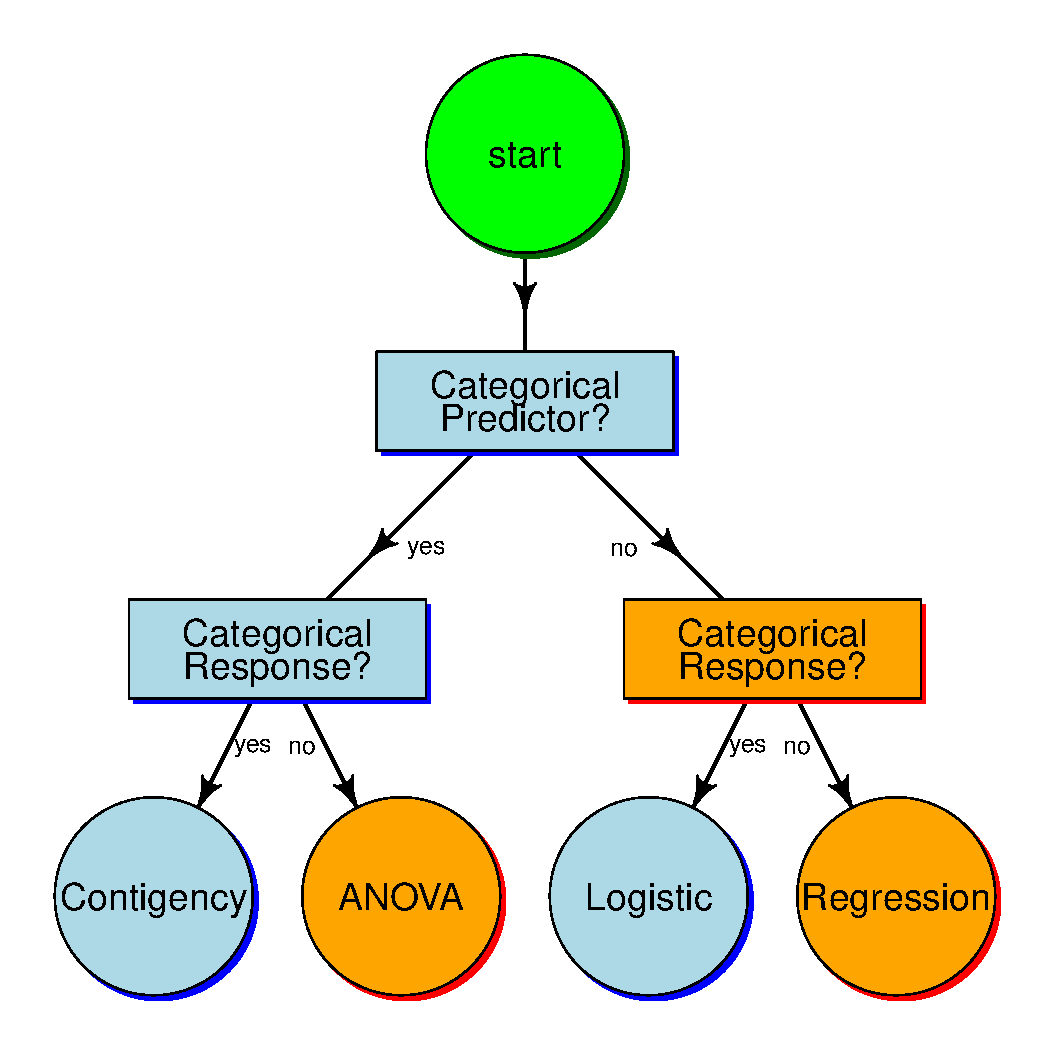
\includegraphics[width=\maxwidth]{figure/unnamed-chunk-3-1} 

\end{knitrout}
\end{center}
\end{figure}

\subsection{Four Frequentists Approaches}

Table \ref{tab:2X2Matrix} describes the statistical approaches available to freqentists in relation to the characteristics of the data. 

\begin{table}
	\caption{2 x 2 Matrix of Inference Methods  --Going to insert graphics to give little pics of analysis...}
	\label{tab:2X2Matrix}
	
		\begin{tabular}{|l|l||ll|} \hline
				&	& \multicolumn{2}{c|}{Response}    \\ \hline
				&			& Categorical 		& Continuous \\ \hline\hline
				
	\parbox[t]{2mm}{\multirow{2}{*}{\rotatebox[origin=c]{90}{Predictor}}} & Categorical 		& Tests of Association	& ANOVA 						\\ 
	&& 
\includegraphics[scale=.05]{../graphics/smoking-non-sequitur.jpg} & \\
			& Continuous				&	Logistic Regression		& Linear Regression	\\ 
	&&& \\ \hline
		\end{tabular}

\end{table}

In our example, the temperature is obviously continuous. Date can be treated as continuous when their are lots of them, but as describe below, it might also be considered categorical -- in part because it's 'ordered' and it's divisible by day -- and not finer resolution, which is decidedly not continuous. However, because there are so many in these records, we can ignore that to continue our analysis. 

\subsection{Data Quality Over Time}

The results of all ecological studies, including time-series designs should be interpreted with caution because subtle problems can haunt the results:\footnote{These need to be revised...not completely appropriate.}

\begin{itemize}
  \item Data on exposure and outcome may be collected in different ways for different populations;
  \item Studies usually rely on routine data sources, which may have been collected for other purposes;
  \item Ecological studies do not allow us to answer questions about individual risks.
\end{itemize}

\subsection{Data Source and Metadata}

TBD

\subsection{Evaluating the Structure of Data}



This is analogous to selection a column or row of numbers in Excel to find the mean and you can usually find it by just looking at your spreadsheet to find the data of interest. In R you have to think a bit about what you want. Using the \texttt{str} command is good start, but we could also just look at the top of the observations to see which variables are of interest. To this we use the function \texttt{head()}, which is short for header, which shows the variable names and the first six observations.

\begin{knitrout}
\definecolor{shadecolor}{rgb}{0.969, 0.969, 0.969}\color{fgcolor}\begin{kframe}
\begin{alltt}
\hlkwd{head}\hlstd{(Thailand)}
\end{alltt}
\begin{verbatim}
##             STATION STATION_NAME     DATE  PRCP TAVG TMAX
## 1 GHCND:TH000048456 DON MUANG TH 19430101 -9999 27.6 33.9
## 2 GHCND:TH000048456 DON MUANG TH 19430102 -9999 26.8 31.7
## 3 GHCND:TH000048456 DON MUANG TH 19430103 -9999 27.2 32.8
## 4 GHCND:TH000048456 DON MUANG TH 19430104 -9999 27.3 33.3
## 5 GHCND:TH000048456 DON MUANG TH 19430105 -9999 27.8 32.2
## 6 GHCND:TH000048456 DON MUANG TH 19430106 -9999 27.1 32.8
##   TMIN    NewDate
## 1   NA 1943-01-01
## 2 21.7 1943-01-02
## 3 21.1 1943-01-03
## 4 21.1 1943-01-04
## 5 21.1 1943-01-05
## 6 21.1 1943-01-06
\end{verbatim}
\end{kframe}
\end{knitrout}


\subsection{Evaluating for Completeness}

NA is the R symbol for missing data and R requires the user to be fairly intentional about how to deal with missing data. Missing data usually mean the dataset is biased. In contrast to many software packages, R forces you to acknowledge the implications of missing data, which can be annoying, like a parent reminding you to clean your room or brush your teeth or take a shower once in the while. But the trade is worth it: you have dealt explicitly with missing data.


\subsection{Evaluating the Central Tendencies}

One of the first things you should do with your data is determine some of the central tendencies. For example, the mean, median, and standard deviation. Also some graphing of the data is also important. For example, what does the distribution of the data look like?

Let's start with the easy stuff. We want to get the mean of the maximum temperatures. That means we need to get the values, named TMAX from the data frame. 

Okay, so we want ``average.'' But typing average by itself doesn't show us anything except an error. Let's try \texttt{str} again. Notice the dollar symbols.  These symbols are use to signify a list of values inside the data frame. To access this list, we type

\begin{knitrout}
\definecolor{shadecolor}{rgb}{0.969, 0.969, 0.969}\color{fgcolor}\begin{kframe}
\begin{alltt}
\hlstd{Thailand}\hlopt{$}\hlstd{TMAX}
\end{alltt}
\end{kframe}
\end{knitrout}

So, now we can get the number of observations, i.e. the length of the vector, by typing

\begin{knitrout}
\definecolor{shadecolor}{rgb}{0.969, 0.969, 0.969}\color{fgcolor}\begin{kframe}
\begin{alltt}
\hlkwd{length}\hlstd{(Thailand}\hlopt{$}\hlstd{TMAX)}
\end{alltt}
\begin{verbatim}
## [1] 27026
\end{verbatim}
\end{kframe}
\end{knitrout}

Okay, let's calculate the mean. In this case, it requires caution. Notice there are NAs in the data. 

Typing \texttt{mean(Thailand\$TMAX)} gives an a ambiguous result, \texttt{NA}. Try it. R is basically saying that the mean can not be calculated because of missing values, thus the mean is also missing. So, can we not calculate the mean when data are missing?  No, we just have to tell R what to do with missing data.  In this case, we tell R to remove them, with the argument \texttt{na.rm="TRUE"}, where True can be abbreviated to T. na.rm="TRUE" roughly translates to 'please remove all the NAs.' 

Okay as of \today, the average is 32.9461248\footnote{How many significant figures should you report? Have I reported this correctly?}. It will change next month when May 2010 is added to the data set. 
Now let's determine the median and standard deviation.

\begin{knitrout}
\definecolor{shadecolor}{rgb}{0.969, 0.969, 0.969}\color{fgcolor}\begin{kframe}
\begin{alltt}
\hlkwd{median}\hlstd{(Thailand}\hlopt{$}\hlstd{TMAX,} \hlkwc{na.rm}\hlstd{=T)}
\end{alltt}
\begin{verbatim}
## [1] 33
\end{verbatim}
\begin{alltt}
\hlkwd{sd}\hlstd{(Thailand}\hlopt{$}\hlstd{TMAX,} \hlkwc{na.rm}\hlstd{=T)}
\end{alltt}
\begin{verbatim}
## [1] 2.336892
\end{verbatim}
\end{kframe}
\end{knitrout}

If you would like a summary of each of the variables, the function is pretty easy to remember--but the output is not exceptionally pleasing. 



\begin{knitrout}
\definecolor{shadecolor}{rgb}{0.969, 0.969, 0.969}\color{fgcolor}\begin{kframe}
\begin{alltt}
\hlkwd{summary}\hlstd{(Thailand)}
\end{alltt}
\begin{verbatim}
##               STATION            STATION_NAME        DATE         
##  GHCND:TH000048456:27026   DON MUANG TH:27026   Min.   :19430101  
##                                                 1st Qu.:19610848  
##                                                 Median :19800265  
##                                                 Mean   :19797426  
##                                                 3rd Qu.:19980830  
##                                                 Max.   :20170630  
##                                                                   
##       PRCP              TAVG              TMAX            TMIN      
##  Min.   :-9999.0   Min.   :-9999.0   Min.   :19.30   Min.   : 2.40  
##  1st Qu.:    0.0   1st Qu.:   27.1   1st Qu.:31.60   1st Qu.:23.00  
##  Median :    0.0   Median :   28.4   Median :33.00   Median :24.50  
##  Mean   :-1532.3   Mean   : -255.2   Mean   :32.95   Mean   :24.02  
##  3rd Qu.:    1.0   3rd Qu.:   29.6   3rd Qu.:34.40   3rd Qu.:25.60  
##  Max.   :  484.1   Max.   :   34.4   Max.   :40.80   Max.   :30.10  
##                                      NA's   :5066    NA's   :7760   
##     NewDate          
##  Min.   :1943-01-01  
##  1st Qu.:1961-08-31  
##  Median :1980-02-29  
##  Mean   :1980-03-04  
##  3rd Qu.:1998-08-29  
##  Max.   :2017-06-30  
## 
\end{verbatim}
\end{kframe}
\end{knitrout}



Nevertheless, the output gives you a really good idea regarding the central tendencies of the entire data set.  Granted typing code might seem like a major step backwards in the computer world, but after a few weeks you will appreciate not having the search through arcane menus to find which button to push--even worse, in these push-button software systems, it often hard to figure out what they are doing. In the case of R, you have a really good idea of what it did, but were much more engaged in the process.

\subsection{Evaluating Spread}

When the mean and median diverge, it means that the distribution is skewed in some way. Let's see what the distribution looks like by creating a histogram.

\begin{verbatim}
hist(Thailand$TMAX)
\end{verbatim}

The one you have made probably does not look that pretty, but with some more advanced coding, this is what it might look like (Figure \ref{fig:histogram}). 

% Additional LaTeX code to add caption to figure
\begin{figure}[h]%
\begin{center}
% \setkeys{Gin}{width=0.75\textwidth} % LaTeX code to read the graphic file in at 75% of its original size

% R code chunk that produces a graphic
\begin{knitrout}
\definecolor{shadecolor}{rgb}{0.969, 0.969, 0.969}\color{fgcolor}
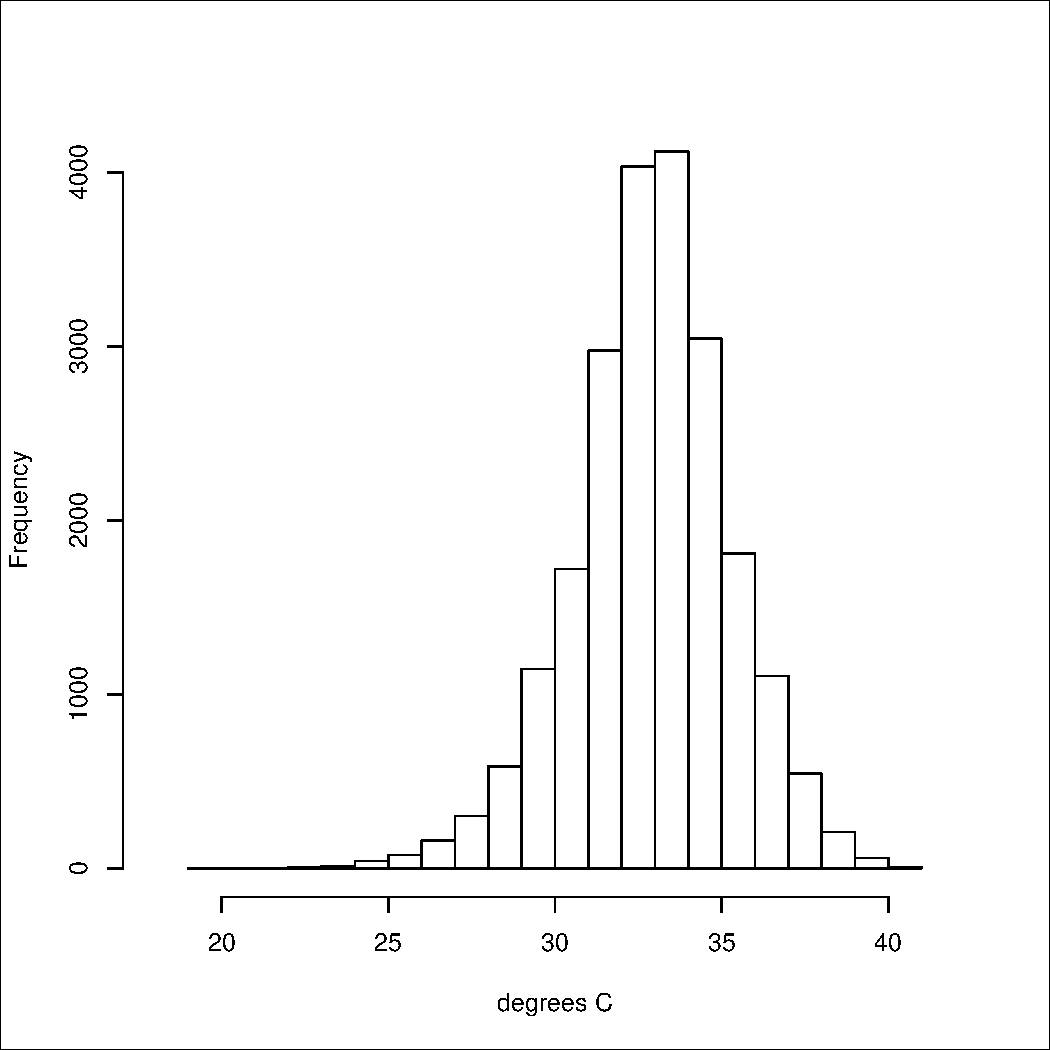
\includegraphics[width=\maxwidth]{figure/fig:histogram-1} 

\end{knitrout}
\caption{Histogram of Maximum Temperatures, Bangkok, Thailand.}
\label{fig:histogram}
\end{center}
\end{figure}

Congratulations, you have made it through the next step in R!  You now know how to do an exploratory analysis and even generate a basic histogram to view the distribution of a data set. Next, we use a standard statistical technique to determine the slope of the line and weather the line is statistically significant-- but first we need to understand something about hypothesis testing.

\subsection{'Null Hypotheses' as the Foundation of Frequentist Statistics}








\subsection{Type I and Type II Errors}

\begin{table}
	\caption{2 x 2 Matrix of Inference Methods  --Going to insert graphics to give little pics of analysis...}
	\label{tab:TypeErrors}
	
		\begin{tabular}{|l|l||ll|} \hline
				&	& \multicolumn{2}{c|}{Reality}    \\ \hline
				&			& Truth 		& Not True \\ \hline\hline
				
	\parbox[t]{2mm}{\multirow{2}{*}{\rotatebox[origin=c]{90}{Statistical Result}}} & 
	Belief & Correct Decision	& Type I 						\\ 
	&& 
\includegraphics[scale=.05]{../graphics/smoking-non-sequitur.jpg} & \\
			& Non-belief				&	Type II		& Correct Decision	\\ 
	&&& \\ \hline
		\end{tabular}

\end{table}

\subsection{Mathematical Mechanisms to Test Hypothesis}

Using the linear model, we can analyze several types of data, when the response variable is continuous. If the have a predictor variable that is categorical, then we often analyze the data using the method known as analysis of variance or ANOVA. If the predictor variable is continuous, then we often analyze data using a regression analysis.

\section{Linear Models in R}

The use of the linear model is the cornerstone of statistics. So ubiquitous it is rarely explained coherently. The linear model can be summarized at the equation for a line, but with the addition of error. You are probably familiar with the equation for a line where, 

\begin{equation}
y = m * x + b
\end{equation}

This equation defines a line, where $m$ is the slope, $b$ is the y-intercept, and the x and y are coordinates. The linear model is based on this form and is usually written as  

\begin{equation}
y \sim \alpha + \beta * x + \epsilon
\end{equation}

The order is usually changed, where the intercept is first, followed by the slope and x variable and the addition of error or noise. The error is usually symbolized as $\epsilon$. In general, in a statistical model, Greek letters are used and instead of an equals sign, we use a tilde, meaning that that left side of the equation is a function of the right side. Luckily, this is the approximate form that R expects, so if you understand this, you will have a pretty good idea of how to code a linear model in R. 

The function to build a linear model is \texttt{lm()}. This function is extremely powerful and can be easily implemented, but this is a good time to see what the help menus look like in R. 

\begin{knitrout}
\definecolor{shadecolor}{rgb}{0.969, 0.969, 0.969}\color{fgcolor}\begin{kframe}
\begin{alltt}
\hlkwd{help}\hlstd{(lm)}
\end{alltt}
\end{kframe}
\end{knitrout}

I am not showing it here, but you should see a long complex looking help page window pop up. All help files in R are structured the same way, so in spite of the uninterpretable text, written by and for computer programmers, the structure will become familiar. Beginning with the description, the help screen describes the function, how to use it, and give some examples. Admittedly, I rarely understand much of the text, but I find the examples to be very useful! In fact, I suggest you paste the example into R and see what happens, I find this one of the best ways to learn R. Use an example that I know works, then change it to make it do what I want it to do.

\section{Linear Regression}

\subsection{What is Linear Regression?}

Linear regression is the most basic and commonly used predictive analysis.  Regression estimates are used to describe data and to explain the relationship between one dependent variable and one or more independent variables.  At the center of the regression analysis is the task of fitting a single line through a scatter plot.  The simplest form with one dependent and one independent variable is defined by the formula:

\begin{equation}
y = a + b*x.
\end{equation}

Sometimes the dependent variable is also called the response.  The independent variables are also predictor variables.  However, Linear Regression Analysis consists of more than just fitting a linear line through a cloud of data points.  It consists of 3 stages:

\begin{enumerate}
  \item analyzing the correlation and directionality of the data, 
  \item estimating the model, i.e., fitting the line, and 
  \item evaluating the validity and usefulness of the model.
\end{enumerate}

There are three major uses for Regression Analysis: 1) causal analysis, 2) forecasting an effect, 3) trend forecasting.  Other than correlation analysis, which focuses on the strength of the relationship between two or more variables, regression analysis assumes a dependence or causal relationship between one or more independent and one dependent variable.

Firstly, it might be used to identify the strength of the effect that the independent variable(s) have on a dependent variable.  Typical questions are what is the strength of relationship between dose and effect, sales and marketing spending, age and income.

Secondly, it can be used to forecast effects or impacts of changes.  That is, regression analysis helps us to understand how much the dependent variable will change when we change one or more independent variables.  Typical questions are, “How much additional Y do I get for one additional unit of X?”.

Thirdly, regression analysis predicts trends and future values.  The regression analysis can be used to get point estimates.  Typical questions are, ``What will the price for gold be 6 month from now?'' ``What is the total effort for a tasks?''

\subsection{Assumptions of Regression}

\subsubsection{Time Series as Ordered Data}

Time series data have a natural temporal ordering. This makes time series analysis distinct from other common data analysis problems.

\subsection{Regression and Climate Change}

One of the ourcomes of the linear regression is to estimate the best fit line

\begin{equation}
y = mx + b + \epsilon,
\end{equation}

where $\epsilon$ is an estimate of the error. In addition, two other estimates are provided, one for the slope, $m$, and the y-intercept, $b$. 

But these estimates are also hypotheses, where the null hypothesis is:

\begin{description}
  \item[slope is zero] Rejecting the null hypothesis would be support the alternative hypothesis, or the estimate of the slope. 
  \item[y-intercept is zero] Rejecting the null hypothesis would support the alternative hypothesis, the estimate of the y-intercept.
\end{description}

Okay, let's see if we can do this for our Bangkok data. Let's test if there is a significant change of daily maximum temperatures (TMAX) with time. Thus, in general terms, Maximum temperature is a function of time, or $TMAX = f(Time)$. 

\begin{equation}
TMAX \sim \alpha + \beta * time + \epsilon
\end{equation}

Translating this in R will take some additional tricks besides just getting the code figured out. First, we need to identify the predictor variable, 'NewDate', in the data frame which we created in SOP85. 

Because these data are in a time series, they are serially correlated, meaning that the June sample will be more like the July sample than the August sample. In addition, the June 2010 sample will be similar to the June 2009 sample. These correlation violate the assumption of independence, but for now, we will ignore this violation and just create a linear model in bliss. 

For the response variable, we will use the daily maximum temeratures, TMAX. Remember there are some missing data, it will be interesting to note how R deals with that.

First, let's create a plot of data using \texttt{plot()}, whose format is \texttt{plot(x, y)} or \texttt{plot(y ~ x)}. We will use the later for now, 

\begin{figure}
\label{fig:test12}
\caption{Maximum daily temperatures for Bangkok, Thailand.}
\begin{knitrout}
\definecolor{shadecolor}{rgb}{0.969, 0.969, 0.969}\color{fgcolor}
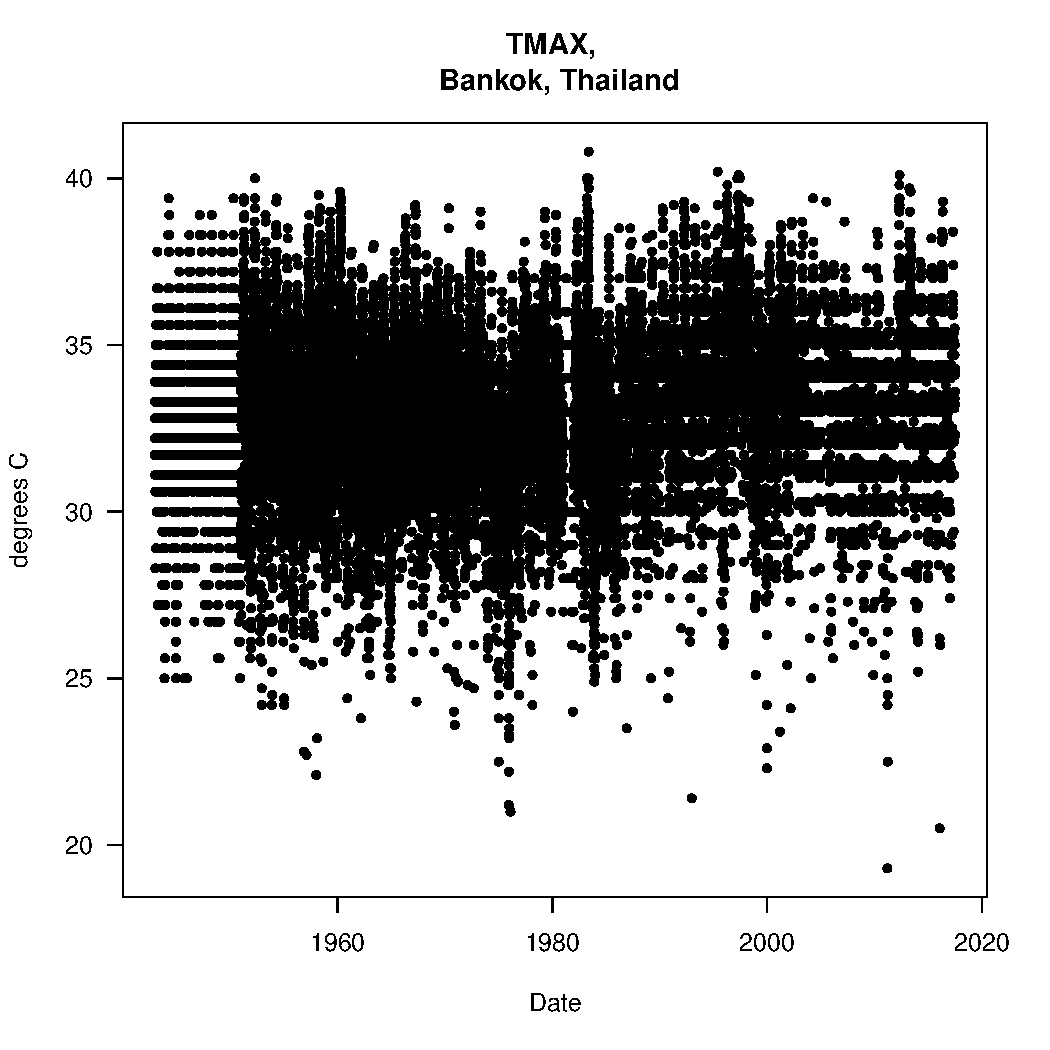
\includegraphics[width=\maxwidth]{figure/Tmaxplot-1} 

\end{knitrout}
\end{figure}

Finally, there is one important difference between the linear model that we used in the \texttt{aov()} function. This time we use the \texttt{lm()} function that arrange the results more in-line with a regression model.
This syntax is still pretty straight forward,  

\begin{knitrout}
\definecolor{shadecolor}{rgb}{0.969, 0.969, 0.969}\color{fgcolor}\begin{kframe}
\begin{alltt}
\hlkwd{lm}\hlstd{(TMAX} \hlopt{~} \hlstd{NewDate,} \hlkwc{data}\hlstd{=Thailand)}
\end{alltt}
\begin{verbatim}
## 
## Call:
## lm(formula = TMAX ~ NewDate, data = Thailand)
## 
## Coefficients:
## (Intercept)      NewDate  
##   3.289e+01    2.702e-05
\end{verbatim}
\end{kframe}
\end{knitrout}

From this model, we learn that the change in $TMAX$ is 
0 degrees $year^{-1}$. Figure~\ref{fig:TMAX_trend} shows a trend of increasing maximum temperatures.

% Additional LaTeX code to add caption to figure
\begin{figure}
\label{fig:TMAX_trend}
\caption{Maximum Daily Temperatures in Bangkok, Thailand.}
\begin{knitrout}
\definecolor{shadecolor}{rgb}{0.969, 0.969, 0.969}\color{fgcolor}
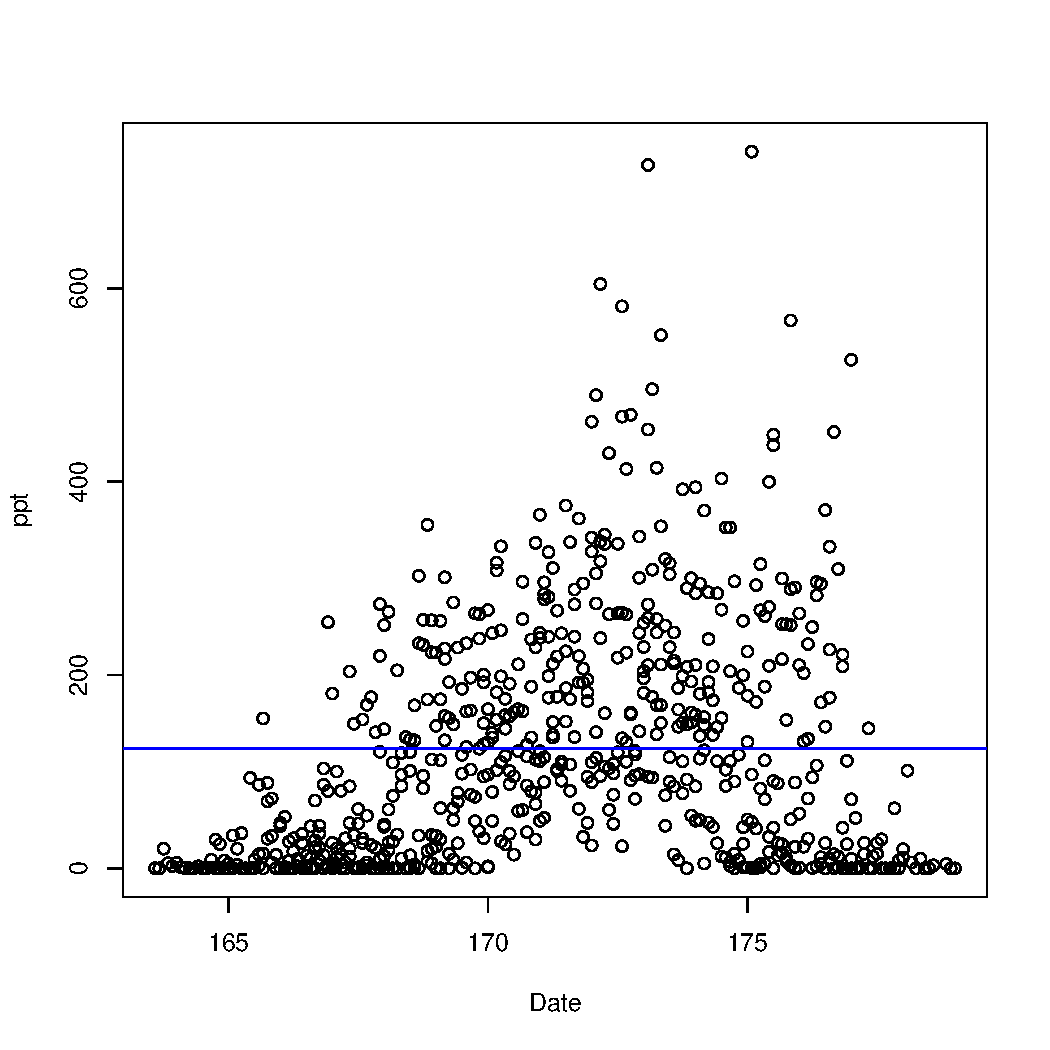
\includegraphics[width=\maxwidth]{figure/unnamed-chunk-12-1} 

\end{knitrout}
\end{figure}

Now determine test the null hypotheses and use the \texttt{summary()} function to display many of the important regression results.

\begin{knitrout}
\definecolor{shadecolor}{rgb}{0.969, 0.969, 0.969}\color{fgcolor}\begin{kframe}
\begin{alltt}
\hlkwd{summary}\hlstd{(}\hlkwd{lm}\hlstd{(TMAX} \hlopt{~} \hlstd{NewDate,} \hlkwc{data}\hlstd{=Thailand))}
\end{alltt}
\begin{verbatim}
## 
## Call:
## lm(formula = TMAX ~ NewDate, data = Thailand)
## 
## Residuals:
##      Min       1Q   Median       3Q      Max 
## -13.9974  -1.3193   0.0782   1.4717   7.7771 
## 
## Coefficients:
##              Estimate Std. Error t value Pr(>|t|)    
## (Intercept) 3.289e+01  1.631e-02 2016.35   <2e-16 ***
## NewDate     2.702e-05  2.140e-06   12.62   <2e-16 ***
## ---
## Signif. codes:  
## 0 '***' 0.001 '**' 0.01 '*' 0.05 '.' 0.1 ' ' 1
## 
## Residual standard error: 2.329 on 21958 degrees of freedom
##   (5066 observations deleted due to missingness)
## Multiple R-squared:  0.007202,	Adjusted R-squared:  0.007157 
## F-statistic: 159.3 on 1 and 21958 DF,  p-value: < 2.2e-16
\end{verbatim}
\end{kframe}
\end{knitrout}

Based on the results, we reject the null hypotheses, i.e. the events that this might occur by chance is small: 2x10$^{-16}$ for the slope is zero and p < 2x10$^{-16}$ for the y-intercept is zero. 

In addition, we have some information on the residuals, and $R^2$ estimates, which are important to interpret the model. 

For now, we can appreciate the the temperature is changing, i.e. increasing, with a slope of 2.7x10$^{-5}$ degrees C per year. 

\subsection{Creating Monthly Averages of Daily Maximum Temperatures}

One of the first things to note is how messy the data look and there are lots of sources of variation. For example, we expect months to respond differently to the climate change. To assess this, we will now analyze the data for monthly means of the maximum temperatures.

\subsection{Creating Monthly Means}

To create monthly means, we need to disagragate the NewDate variable into a month and year variables.

First we can use the \texttt{as.Date()} function to extract a portion of the date, where \%m is for month and \%Y is for a four digit year. Then, we create new variables in our dataframe, one for month and one for year.

\begin{knitrout}
\definecolor{shadecolor}{rgb}{0.969, 0.969, 0.969}\color{fgcolor}\begin{kframe}
\begin{alltt}
\hlstd{Thailand}\hlopt{$}\hlstd{Month} \hlkwb{=} \hlkwd{format}\hlstd{(}\hlkwd{as.Date}\hlstd{(Thailand}\hlopt{$}\hlstd{NewDate),} \hlkwc{format} \hlstd{=} \hlstr{"%m"}\hlstd{)}
\hlstd{Thailand}\hlopt{$}\hlstd{Year} \hlkwb{=} \hlkwd{format}\hlstd{(Thailand}\hlopt{$}\hlstd{NewDate,} \hlkwc{format}\hlstd{=}\hlstr{"%Y"}\hlstd{)}
\end{alltt}
\end{kframe}
\end{knitrout}

After creating the month and year as separate variables, we can use them to caculate the mean using the \texttt{aggregate()} function. In the code below, we can also calculate the standard deviation too, although I haven't used this measure in this document, several students have asked for this for their analysis.

\begin{knitrout}
\definecolor{shadecolor}{rgb}{0.969, 0.969, 0.969}\color{fgcolor}\begin{kframe}
\begin{alltt}
\hlstd{MonthlyTMAXMean} \hlkwb{=} \hlkwd{aggregate}\hlstd{(TMAX} \hlopt{~} \hlstd{Month} \hlopt{+} \hlstd{Year, Thailand, mean)}

\hlstd{MonthlyTMAXMean}\hlopt{$}\hlstd{YEAR} \hlkwb{=} \hlkwd{as.numeric}\hlstd{(MonthlyTMAXMean}\hlopt{$}\hlstd{Year)}
\hlstd{MonthlyTMAXMean}\hlopt{$}\hlstd{MONTH} \hlkwb{=} \hlkwd{as.numeric}\hlstd{(MonthlyTMAXMean}\hlopt{$}\hlstd{Month)}
\hlkwd{str}\hlstd{(MonthlyTMAXMean)}
\end{alltt}
\begin{verbatim}
## 'data.frame':	888 obs. of  5 variables:
##  $ Month: chr  "01" "02" "03" "04" ...
##  $ Year : chr  "1943" "1943" "1943" "1943" ...
##  $ TMAX : num  32.2 33.2 34.9 33.5 33.8 ...
##  $ YEAR : num  1943 1943 1943 1943 1943 ...
##  $ MONTH: num  1 2 3 4 5 6 7 8 9 10 ...
\end{verbatim}
\begin{alltt}
\hlstd{MonthlyTMAXSD} \hlkwb{=} \hlkwd{aggregate}\hlstd{(TMAX} \hlopt{~} \hlstd{Month} \hlopt{+} \hlstd{Year, Thailand, sd)}

\hlstd{MonthlyTMAXSD}\hlopt{$}\hlstd{YEAR} \hlkwb{=} \hlkwd{as.numeric}\hlstd{(MonthlyTMAXSD}\hlopt{$}\hlstd{Year)}
\hlstd{MonthlyTMAXSD}\hlopt{$}\hlstd{MONTH} \hlkwb{=} \hlkwd{as.numeric}\hlstd{(MonthlyTMAXSD}\hlopt{$}\hlstd{Month)}
\hlstd{MonthlyTMAXSD}\hlopt{$}\hlstd{NewDate} \hlkwb{=} \hlstd{MonthlyTMAXSD}\hlopt{$}\hlstd{YEAR} \hlopt{+} \hlstd{(MonthlyTMAXSD}\hlopt{$}\hlstd{MONTH} \hlopt{-} \hlnum{1}\hlstd{)}\hlopt{/}\hlnum{12}

\hlkwd{head}\hlstd{(MonthlyTMAXSD)}
\end{alltt}
\begin{verbatim}
##   Month Year     TMAX YEAR MONTH  NewDate
## 1    01 1943 1.523317 1943     1 1943.000
## 2    02 1943 1.668648 1943     2 1943.083
## 3    03 1943 1.969395 1943     3 1943.167
## 4    04 1943 2.521970 1943     4 1943.250
## 5    05 1943 2.100818 1943     5 1943.333
## 6    06 1943 1.041763 1943     6 1943.417
\end{verbatim}
\end{kframe}
\end{knitrout}

\begin{knitrout}
\definecolor{shadecolor}{rgb}{0.969, 0.969, 0.969}\color{fgcolor}\begin{kframe}
\begin{alltt}
\hlkwd{plot}\hlstd{(MonthlyTMAXMean}\hlopt{$}\hlstd{TMAX,} \hlkwc{ty}\hlstd{=}\hlstr{'l'}\hlstd{)}
\end{alltt}
\end{kframe}
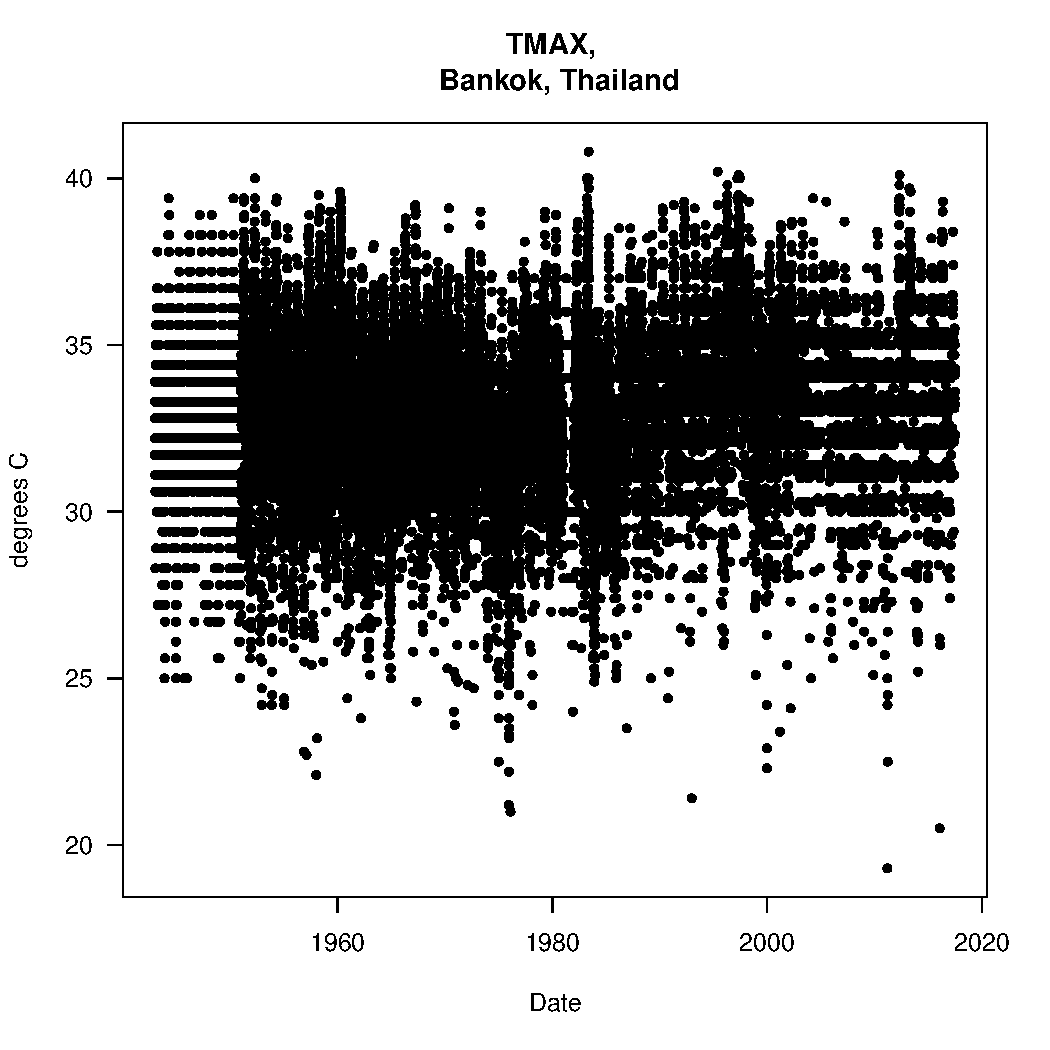
\includegraphics[width=\maxwidth]{figure/unnamed-chunk-13-1} 

\end{knitrout}

Below is Standard Deviation

\begin{knitrout}
\definecolor{shadecolor}{rgb}{0.969, 0.969, 0.969}\color{fgcolor}\begin{kframe}
\begin{alltt}
\hlcom{#plot(MonthlySD$TMAX, ty='l')}

\hlcom{#plot(TMAX~ NewDate, data=MonthlySD, ty='l')}
\hlcom{#SD.lm <- lm(TMAX~NewDate, data=MonthlySD)}
\hlcom{#summary(SD.lm)}

\hlcom{#abline(coef(SD.lm), col="red")}
\end{alltt}
\end{kframe}
\end{knitrout}

Selecting for 1 Month -- May

Perhaps, we can get a better handle on this stuff if we analyze for just one month at a time -- certainly easier to visualize!

\begin{knitrout}
\definecolor{shadecolor}{rgb}{0.969, 0.969, 0.969}\color{fgcolor}\begin{kframe}
\begin{alltt}
\hlcom{#plot(MonthlyTMAXMean$TMAX[MonthlyTMAXMean$Month=="05"], ty='l')}
\hlkwd{plot}\hlstd{(TMAX}\hlopt{~}\hlstd{YEAR,} \hlkwc{data}\hlstd{=MonthlyTMAXMean[MonthlyTMAXMean}\hlopt{$}\hlstd{Month}\hlopt{==}\hlstr{"05"}\hlstd{,],} \hlkwc{ty}\hlstd{=}\hlstr{'l'}\hlstd{,} \hlkwc{xlim}\hlstd{=}\hlkwd{c}\hlstd{(}\hlnum{1950}\hlstd{,} \hlnum{2020}\hlstd{))}
\hlstd{May.lm} \hlkwb{<-} \hlkwd{lm}\hlstd{(TMAX}\hlopt{~}\hlstd{YEAR,} \hlkwc{data}\hlstd{=MonthlyTMAXMean[MonthlyTMAXMean}\hlopt{$}\hlstd{Month}\hlopt{==}\hlstr{"05"}\hlstd{,])}
\hlkwd{summary}\hlstd{(May.lm)}
\end{alltt}
\begin{verbatim}
## 
## Call:
## lm(formula = TMAX ~ YEAR, data = MonthlyTMAXMean[MonthlyTMAXMean$Month == 
##     "05", ])
## 
## Residuals:
##      Min       1Q   Median       3Q      Max 
## -2.85376 -0.93210 -0.04633  0.81231  3.15347 
## 
## Coefficients:
##              Estimate Std. Error t value Pr(>|t|)
## (Intercept) 17.238621  13.753642   1.253    0.214
## YEAR         0.008756   0.006946   1.261    0.211
## 
## Residual standard error: 1.302 on 73 degrees of freedom
## Multiple R-squared:  0.0213,	Adjusted R-squared:  0.007897 
## F-statistic: 1.589 on 1 and 73 DF,  p-value: 0.2115
\end{verbatim}
\begin{alltt}
\hlkwd{abline}\hlstd{(}\hlkwd{coef}\hlstd{(May.lm),} \hlkwc{col}\hlstd{=}\hlstr{"red"}\hlstd{)}
\end{alltt}
\end{kframe}
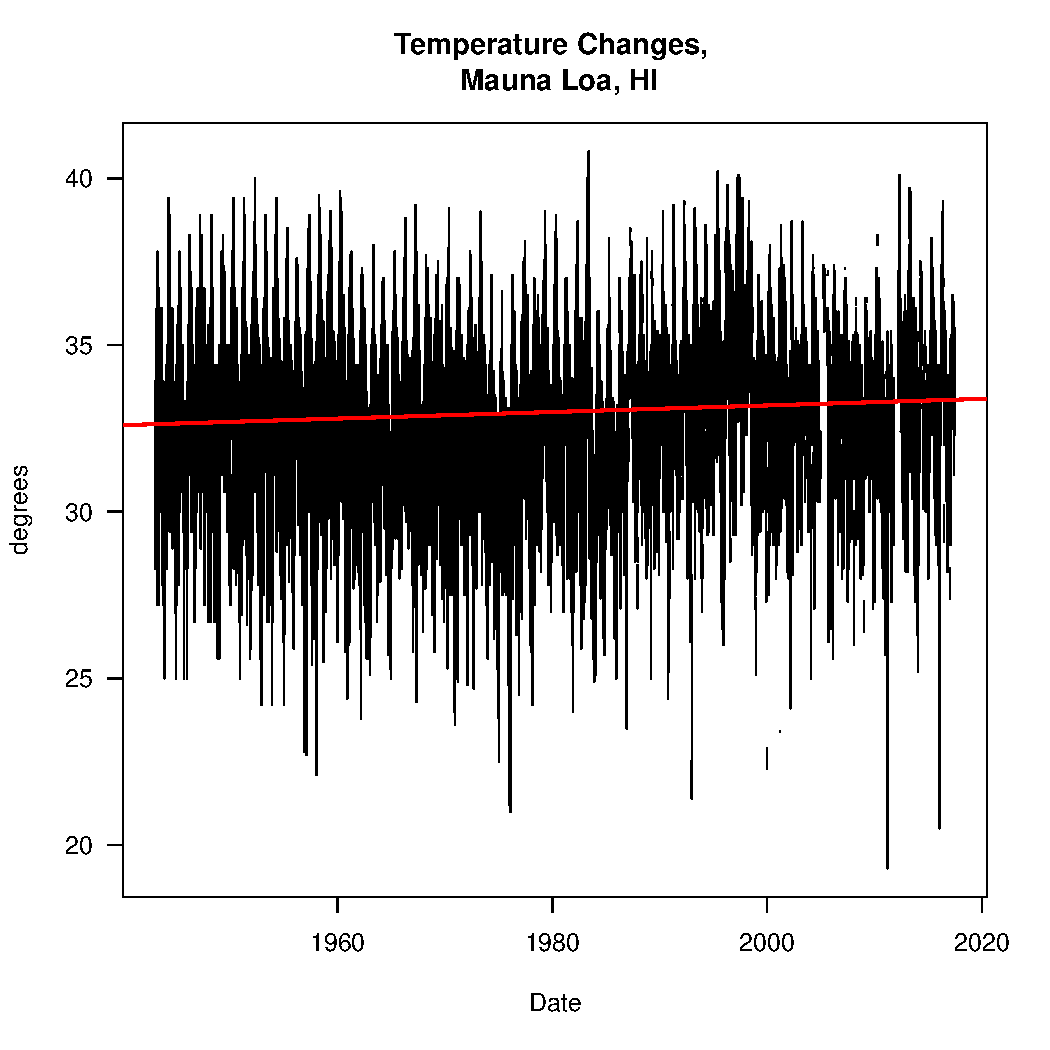
\includegraphics[width=\maxwidth]{figure/unnamed-chunk-15-1} 

\end{knitrout}

Now, the change is 0.0088 degress C/year or 0.876 degress C/100 years with a probability of 0.2115. Although we can't reject the null hypothesis, we find the method to be fairly straightforward! 

%https://feliperego.github.io/blog/2015/10/23/Interpreting-Model-Output-In-R

\subsection{Testing all the Months}

I think you should evaluate every month and see what happens. You might also consider looking at the TMIN as well. Could be important!\footnote{What about multiple hypotheses in one dataset!}

Below, I have create code to evaluate all of the months at once, but you may prefer to go through each month manually and change the number from 5 to other months of the year. 

\begin{figure}
\begin{knitrout}
\definecolor{shadecolor}{rgb}{0.969, 0.969, 0.969}\color{fgcolor}
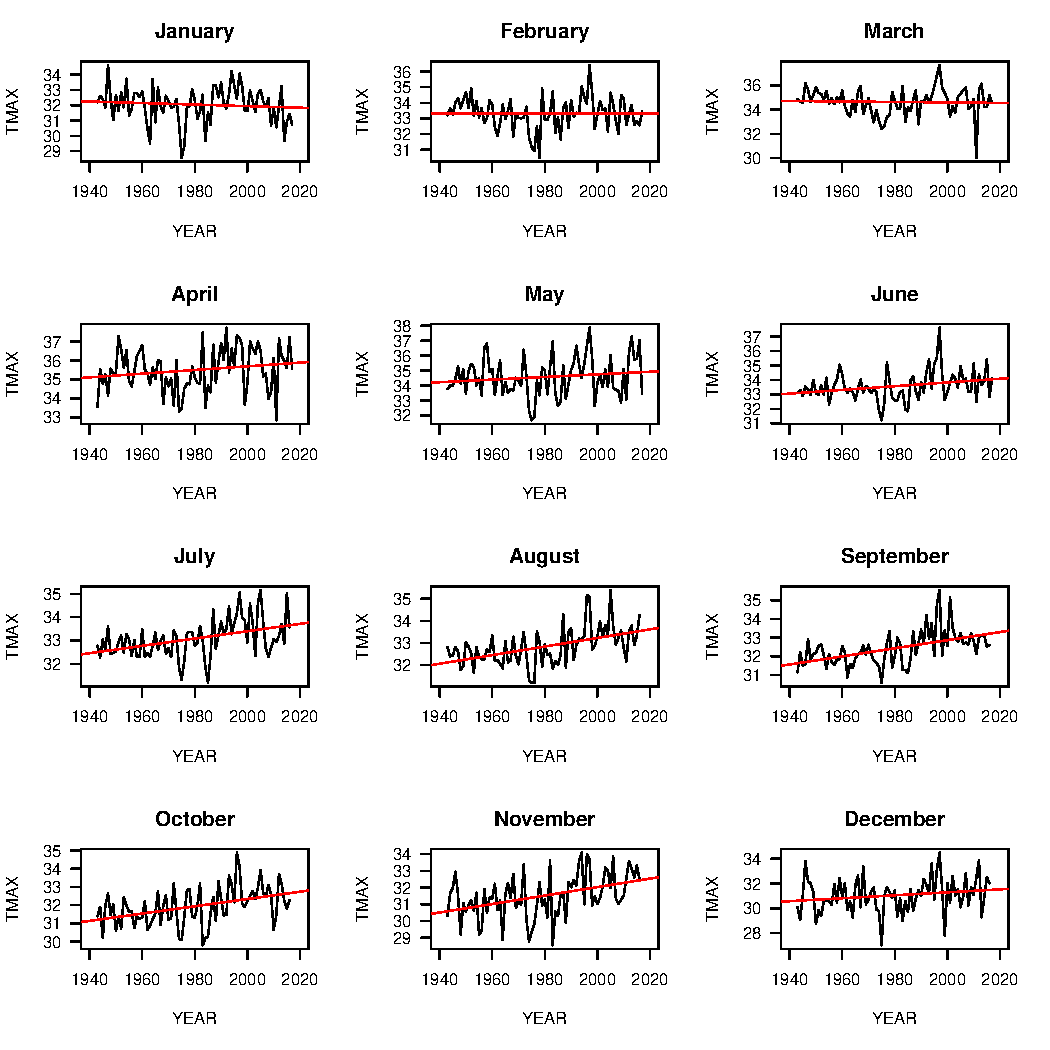
\includegraphics[width=\maxwidth]{figure/12MonthsTMAX-1} 

\end{knitrout}
\end{figure}

\subsection{Next Steps}

\subsubsection{Analyzing Minimum Daily Temperatures}

Alternatively, it might be important to evaluate changes to the daily mininum temperatures. Following the same steps we used before but using the TMIN instead of TMAX, let's analyze the monthly average of daily minimum temperatures by following these steps: 

\begin{enumerate}

\item First, let's plot the daily minimum temperatures, and as with the daily maximum temperatures, find tons of scatter (Table \ref{fig:TMIN_trend}).

% Additional LaTeX code to add caption to figure
\begin{figure}
\label{fig:TMIN_trend}
\caption{Minimum Daily Temperatures in Bangkok, Thailand.}
\begin{knitrout}
\definecolor{shadecolor}{rgb}{0.969, 0.969, 0.969}\color{fgcolor}
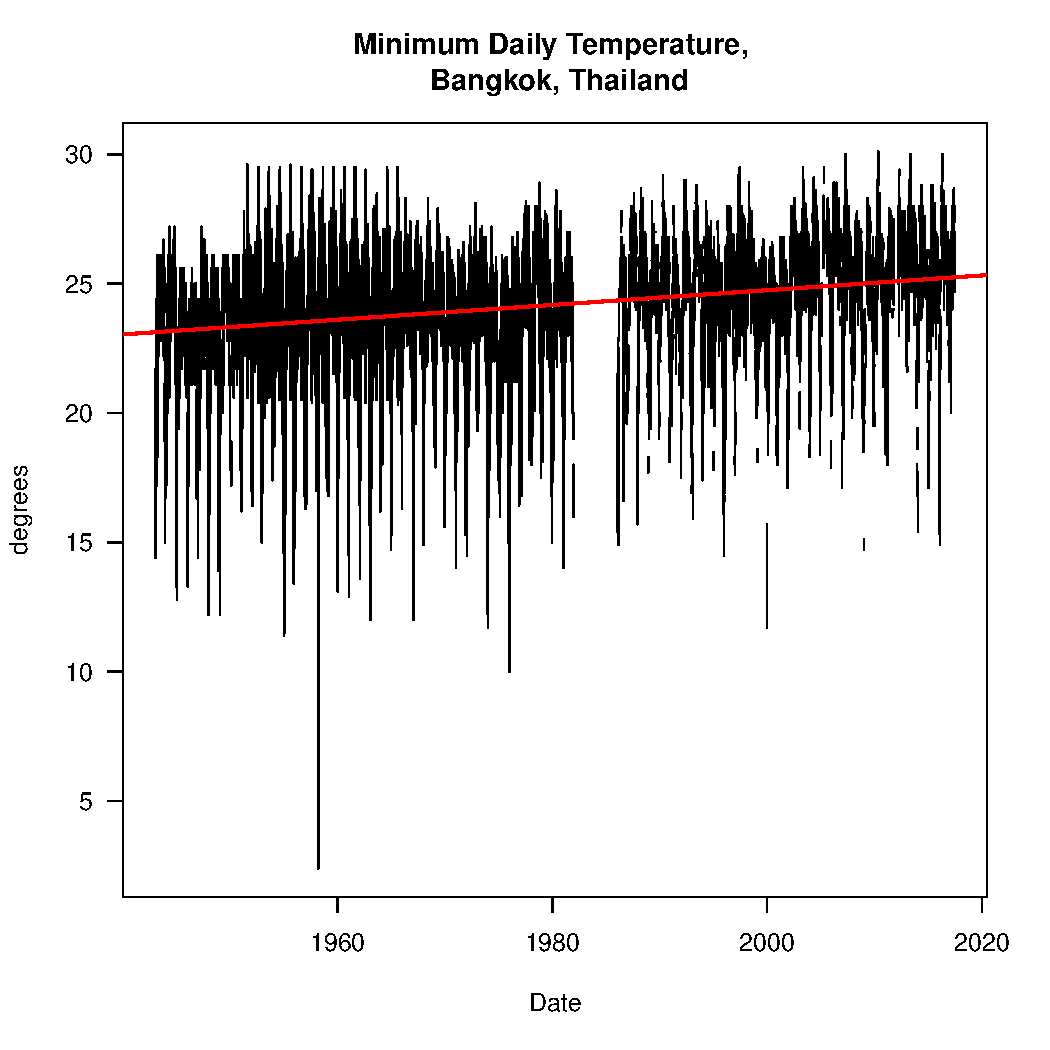
\includegraphics[width=\maxwidth]{figure/unnamed-chunk-16-1} 

\end{knitrout}
\end{figure}

There appears to be a trend, but it's clouded with lots of variation. 

  \item We create a monthly TMIN mean for each month.

\begin{knitrout}
\definecolor{shadecolor}{rgb}{0.969, 0.969, 0.969}\color{fgcolor}\begin{kframe}
\begin{alltt}
\hlstd{MonthlyTMINMean} \hlkwb{=} \hlkwd{aggregate}\hlstd{(TMIN} \hlopt{~} \hlstd{Month} \hlopt{+} \hlstd{Year, Thailand, mean)}

\hlstd{MonthlyTMINMean}\hlopt{$}\hlstd{YEAR} \hlkwb{=} \hlkwd{as.numeric}\hlstd{(MonthlyTMINMean}\hlopt{$}\hlstd{Year)}

\hlcom{# Fixing the Format of Month and Year as numeric}
\hlstd{MonthlyTMINMean}\hlopt{$}\hlstd{YEAR} \hlkwb{=} \hlkwd{as.numeric}\hlstd{(MonthlyTMINMean}\hlopt{$}\hlstd{Year)}
\hlstd{MonthlyTMINMean}\hlopt{$}\hlstd{MONTH} \hlkwb{=} \hlkwd{as.numeric}\hlstd{(MonthlyTMINMean}\hlopt{$}\hlstd{Month)}
\hlkwd{head}\hlstd{(MonthlyTMINMean)}
\end{alltt}
\begin{verbatim}
##   Month Year     TMIN YEAR MONTH
## 1    01 1943 18.54828 1943     1
## 2    02 1943 20.73077 1943     2
## 3    03 1943 23.39655 1943     3
## 4    04 1943 23.79259 1943     4
## 5    05 1943 24.87692 1943     5
## 6    06 1943 24.76429 1943     6
\end{verbatim}
\end{kframe}
\end{knitrout}

\item Create a plot of the monthly average of the daily minimum temperatures. 


\begin{knitrout}
\definecolor{shadecolor}{rgb}{0.969, 0.969, 0.969}\color{fgcolor}\begin{kframe}
\begin{alltt}
\hlkwd{plot}\hlstd{(MonthlyTMINMean}\hlopt{$}\hlstd{TMIN,} \hlkwc{ty}\hlstd{=}\hlstr{'l'}\hlstd{)}
\end{alltt}
\end{kframe}
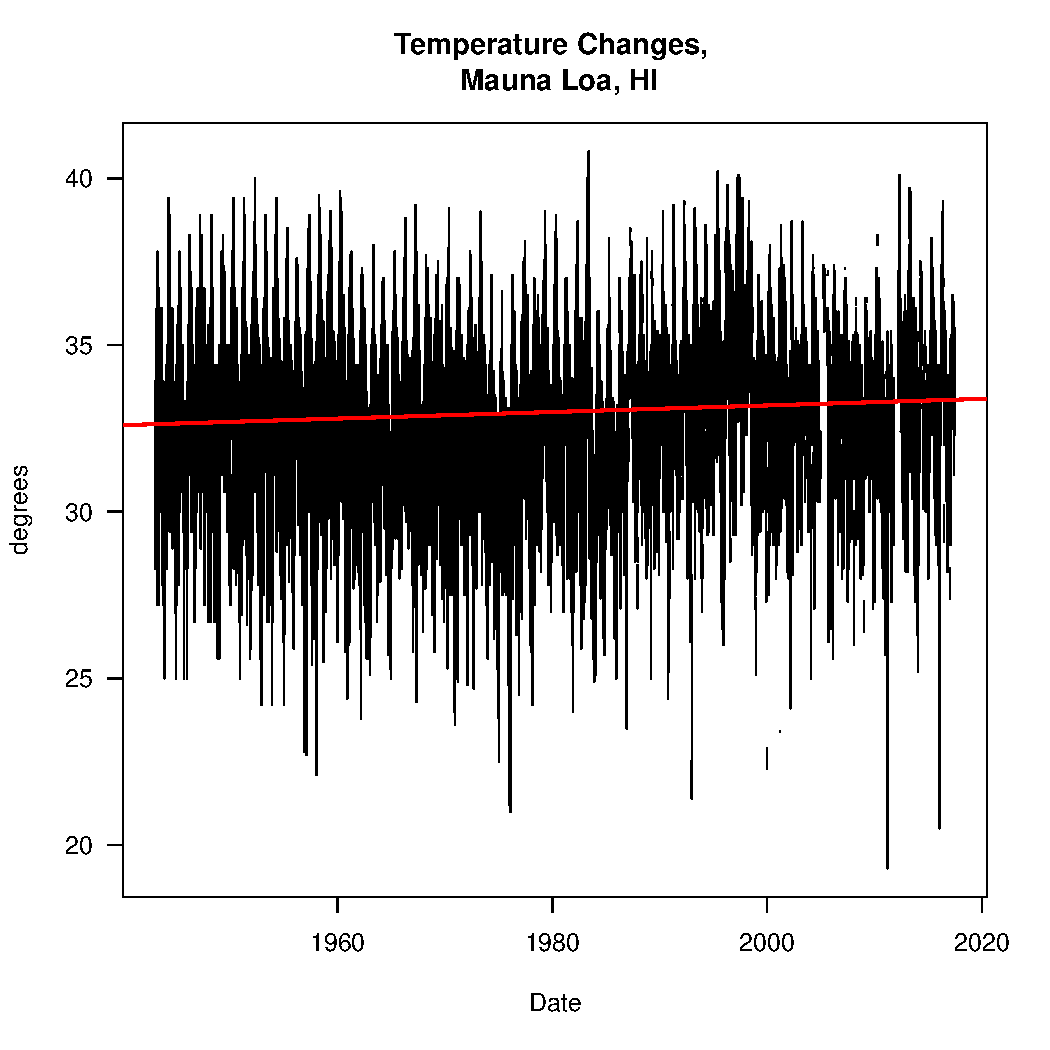
\includegraphics[width=\maxwidth]{figure/unnamed-chunk-17-1} 

\end{knitrout}

There is still lots of scatter and now we can subset our data by month. 

\item Using the example above, we'll plot all 12 months at once to look for patterns (Table \ref{fig:TMIN}).

\begin{figure}[ht]
\caption{Twelve Months of Monthly Average Daily Minimum 
Temperatures, Bangkok, Thailand}
\label{fig:TMIN}
\begin{knitrout}
\definecolor{shadecolor}{rgb}{0.969, 0.969, 0.969}\color{fgcolor}
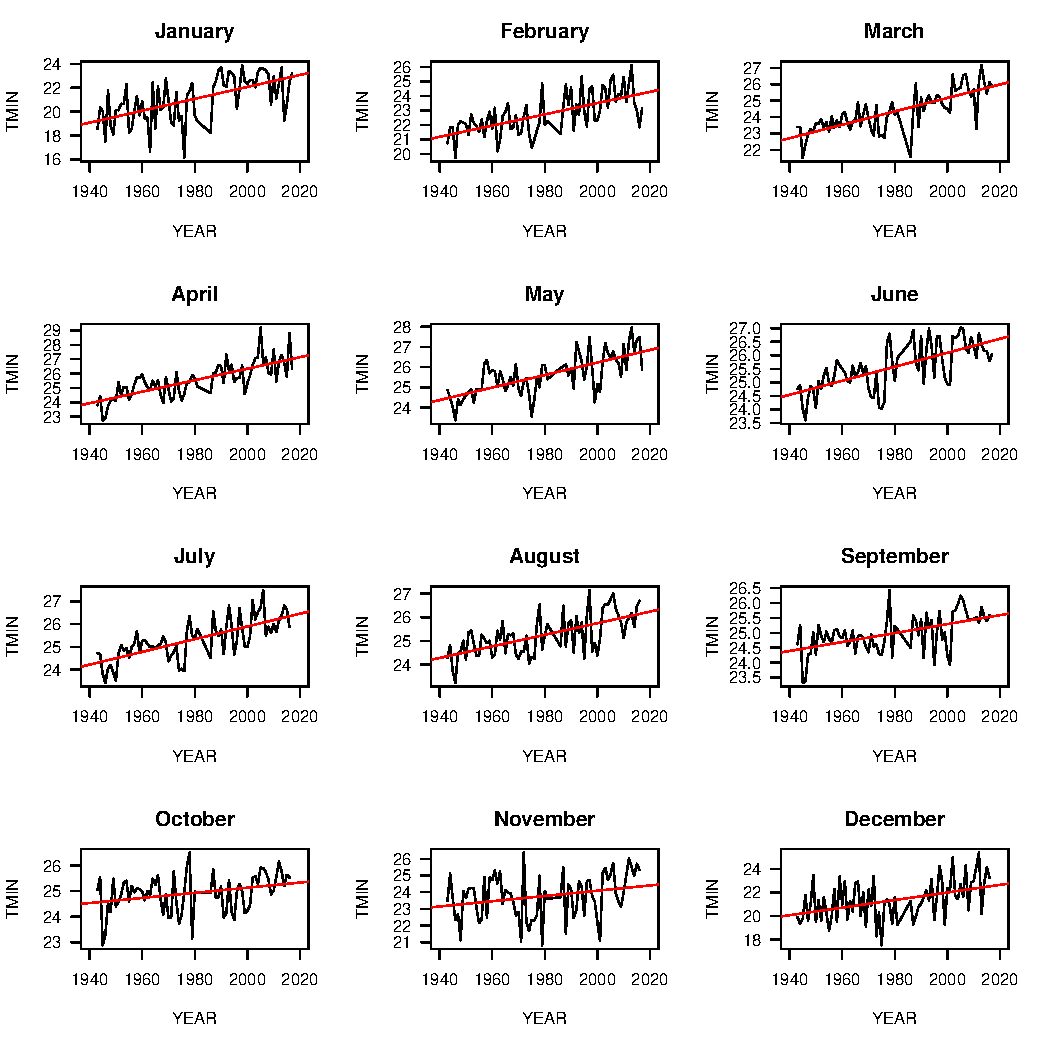
\includegraphics[width=\maxwidth]{figure/12MonthsTMIN-1} 

\end{knitrout}
\end{figure} 

\item The change in minimum temperatures seems to be even more compelling than the maximum temperatures. To compare, look at the Table \ref{tab:results} to appreciate estimated slopes and their associated null hypothesis probabilities. 

\begin{kframe}
\begin{alltt}
\hlkwd{library}\hlstd{(xtable)}
\hlstd{Results} \hlkwb{<-} \hlkwd{data.frame}\hlstd{(}\hlkwc{Month} \hlstd{= TMINresult[}\hlkwd{c}\hlstd{(}\hlnum{2}\hlopt{:}\hlnum{13}\hlstd{),}\hlnum{1}\hlstd{],} \hlkwc{TMINSlope} \hlstd{= TMINresult[}\hlkwd{c}\hlstd{(}\hlnum{2}\hlopt{:}\hlnum{13}\hlstd{),}\hlnum{2}\hlstd{],} \hlkwc{TMIN_P} \hlstd{=} \hlkwd{as.numeric}\hlstd{(TMINresult[}\hlkwd{c}\hlstd{(}\hlnum{2}\hlopt{:}\hlnum{13}\hlstd{),}\hlnum{3}\hlstd{]),} \hlkwc{TMINRsq} \hlstd{= TMINresult[}\hlkwd{c}\hlstd{(}\hlnum{2}\hlopt{:}\hlnum{13}\hlstd{),}\hlnum{4}\hlstd{],} \hlkwc{TMAXSlope} \hlstd{= TMAXresult[}\hlkwd{c}\hlstd{(}\hlnum{2}\hlopt{:}\hlnum{13}\hlstd{),}\hlnum{2}\hlstd{],} \hlkwc{TMAX_P} \hlstd{=} \hlkwd{as.numeric}\hlstd{(TMAXresult[}\hlkwd{c}\hlstd{(}\hlnum{2}\hlopt{:}\hlnum{13}\hlstd{),}\hlnum{3}\hlstd{]),} \hlkwc{TMAXRsq} \hlstd{= TMAXresult[}\hlkwd{c}\hlstd{(}\hlnum{2}\hlopt{:}\hlnum{13}\hlstd{),}\hlnum{4}\hlstd{])}
\hlstd{Results}\hlopt{$}\hlstd{starTMIN} \hlkwb{=} \hlstr{"NS"}
\hlstd{Results}\hlopt{$}\hlstd{starTMIN[Results}\hlopt{$}\hlstd{TMIN_P} \hlopt{<=} \hlnum{.05}\hlstd{]} \hlkwb{=} \hlstr{"*"}
\hlstd{Results}\hlopt{$}\hlstd{starTMIN[Results}\hlopt{$}\hlstd{TMIN_P} \hlopt{<} \hlnum{0.01}\hlstd{]} \hlkwb{=} \hlstr{"**"}
\hlstd{Results}\hlopt{$}\hlstd{starTMIN[Results}\hlopt{$}\hlstd{TMIN_P} \hlopt{<} \hlnum{0.001}\hlstd{]} \hlkwb{=} \hlstr{"***"}
\hlstd{Results}\hlopt{$}\hlstd{starTMAX} \hlkwb{=} \hlstr{"NS"}
\hlstd{Results}\hlopt{$}\hlstd{starTMAX[Results}\hlopt{$}\hlstd{TMAX_P} \hlopt{<} \hlnum{0.05}\hlstd{]} \hlkwb{=} \hlstr{"*"}
\hlstd{Results}\hlopt{$}\hlstd{starTMAX[Results}\hlopt{$}\hlstd{TMAX_P} \hlopt{<} \hlnum{0.01}\hlstd{]} \hlkwb{=} \hlstr{"**"}
\hlstd{Results}\hlopt{$}\hlstd{starTMAX[Results}\hlopt{$}\hlstd{TMAX_P} \hlopt{<} \hlnum{0.001}\hlstd{]} \hlkwb{=} \hlstr{"***"}
\hlstd{Results}\hlopt{$}\hlstd{TMINslope}\hlkwb{=}\hlkwd{paste}\hlstd{(Results}\hlopt{$}\hlstd{TMINSlope, Results}\hlopt{$}\hlstd{starTMIN)}
\hlstd{Results}\hlopt{$}\hlstd{TMAXslope}\hlkwb{=}\hlkwd{paste}\hlstd{(Results}\hlopt{$}\hlstd{TMAXSlope, Results}\hlopt{$}\hlstd{starTMAX)}
\hlkwd{colnames}\hlstd{(Results)} \hlkwb{<-} \hlkwd{c}\hlstd{(}\hlstr{"Month"}\hlstd{,} \hlstr{"2"}\hlstd{,} \hlstr{"3"}\hlstd{,} \hlstr{"R^2"}\hlstd{,} \hlstr{"5"}\hlstd{,} \hlstr{"6"}\hlstd{,} \hlstr{"R^2"}\hlstd{,} \hlstr{"8"}\hlstd{,} \hlstr{"9"}\hlstd{,} \hlstr{"Slope TMIN"}\hlstd{,} \hlstr{"Slope TMAX"}\hlstd{)}
\hlkwd{print}\hlstd{(}\hlkwd{xtable}\hlstd{(Results[,}\hlkwd{c}\hlstd{(}\hlnum{1}\hlstd{,} \hlnum{10}\hlstd{,} \hlnum{4}\hlstd{,} \hlnum{11}\hlstd{,} \hlnum{7}\hlstd{)]))}
\end{alltt}
\end{kframe}% latex table generated in R 3.3.1 by xtable 1.8-2 package
% Mon Jul 10 23:40:15 2017
\begin{table}[ht]
\centering
\begin{tabular}{rlllll}
  \hline
 & Month & Slope TMIN & R\verb|^|2 & Slope TMAX & R\verb|^|2.1 \\ 
  \hline
1 & January & 0.0498 *** & 0.341 & -0.0051 NS & 0.009 \\ 
  2 & February & 0.0387 *** & 0.385 & -1e-04 NS & 0 \\ 
  3 & March & 0.0409 *** & 0.567 & -0.002 NS & 0.001 \\ 
  4 & April & 0.04 *** & 0.551 & 0.0097 NS & 0.035 \\ 
  5 & May & 0.031 *** & 0.48 & 0.0088 NS & 0.021 \\ 
  6 & June & 0.0259 *** & 0.448 & 0.0129 * & 0.078 \\ 
  7 & July & 0.028 *** & 0.493 & 0.0157 *** & 0.173 \\ 
  8 & August & 0.0245 *** & 0.395 & 0.0194 *** & 0.245 \\ 
  9 & September & 0.015 *** & 0.279 & 0.0217 *** & 0.257 \\ 
  10 & October & 0.01 * & 0.093 & 0.02 *** & 0.174 \\ 
  11 & November & 0.0158 * & 0.067 & 0.0253 *** & 0.169 \\ 
  12 & December & 0.0322 *** & 0.178 & 0.0119 NS & 0.034 \\ 
   \hline
\end{tabular}
\end{table}


Based on the results above, the slopes are greatest during the dry season (starting in May) for the maximum temperatures -- but the minimum temperatures show the largest slopes (change) and peaking between January and April.  

In addition, the $r^2$ values signify the amount of the variance explained by the predictor -- in the case of TMIN, most of the values are over 20\% meaning that over 20\% of the variance is explained by time. While in March and April over time explains 50\% of the variance. 

This is very high for uncontroled experiments. However, we should be cognizant that in many cases, especially for the maximum temperatures, it is less than 10\%. This means the the variation in temperature are not predicted by time -- thus, as a modeler, I would work very hard to capture other sources to better understand what is going on in Thailand. 

Finally, we should also be very concerned about testing 2 dozen hypotheses with our little R code. It's easy to do, but based on change alone, with a critical value of 0.05, we should expect 1 in 20 tests to give us a Type I error, a signal when one doesn't exists. Since we did 12 tests, we should expect a good chance that one or more of our tests will reject the null hypothesis incorrectly. Yikes!  
Please keep this in mind and be careful to avoid this potential problem. 

As we might expect, the a small amount of the variance is explained by the ``Month.'' Many things predict temerpature, that year is one, is quite problematic.

\item What we have not determined is the cause. So, be careful when you describe the results, cause and effect cannot be analyzed using this method.

\end{enumerate}

\subsubsection{Precipitation: Departure from Mean}

Precipiation might depend more on the departure from the mean (often referred as as normal, whatever that means!).  I think it's worth pursuing, but haven't finished the analysis yet.

Precipitation is something that might increase or decrease due to climate change. So, to analyze this, we will evaluate how much precipitation has deveated from the mean, by plotting the rainfall and the mean in a time-series plot. 

Second, we need to remove the missing values and evalaute which years have complete years. If you are missing rainy months, then the whole year should be thrown out -- but what about partial years in the drought season? We'll need to be consistent -- assuming that missing data are not zeros, we'll define complete years as over 300 days of data. 

NOTE: The missing values have not been converted to NAs!
\begin{knitrout}
\definecolor{shadecolor}{rgb}{0.969, 0.969, 0.969}\color{fgcolor}\begin{kframe}
\begin{alltt}
\hlstd{Thailand}\hlopt{$}\hlstd{PRCP[Thailand}\hlopt{$}\hlstd{PRCP}\hlopt{==-}\hlnum{9999}\hlstd{]} \hlkwb{<-} \hlnum{NA}

\hlstd{Missing} \hlkwb{<-} \hlkwd{aggregate}\hlstd{(}\hlkwd{is.na}\hlstd{(Thailand}\hlopt{$}\hlstd{PRCP),} \hlkwd{list}\hlstd{(Thailand}\hlopt{$}\hlstd{Month, Thailand}\hlopt{$}\hlstd{Year), sum)}
\hlstd{Missing}\hlopt{$}\hlstd{Date} \hlkwb{=} \hlkwd{as.numeric}\hlstd{(Missing}\hlopt{$}\hlstd{Group.1)} \hlopt{+} \hlkwd{as.numeric}\hlstd{(Missing}\hlopt{$}\hlstd{Group.2)}\hlopt{/}\hlnum{12}
\hlkwd{plot}\hlstd{(x} \hlopt{~} \hlstd{Date,} \hlkwc{data}\hlstd{=Missing)}
\end{alltt}
\end{kframe}
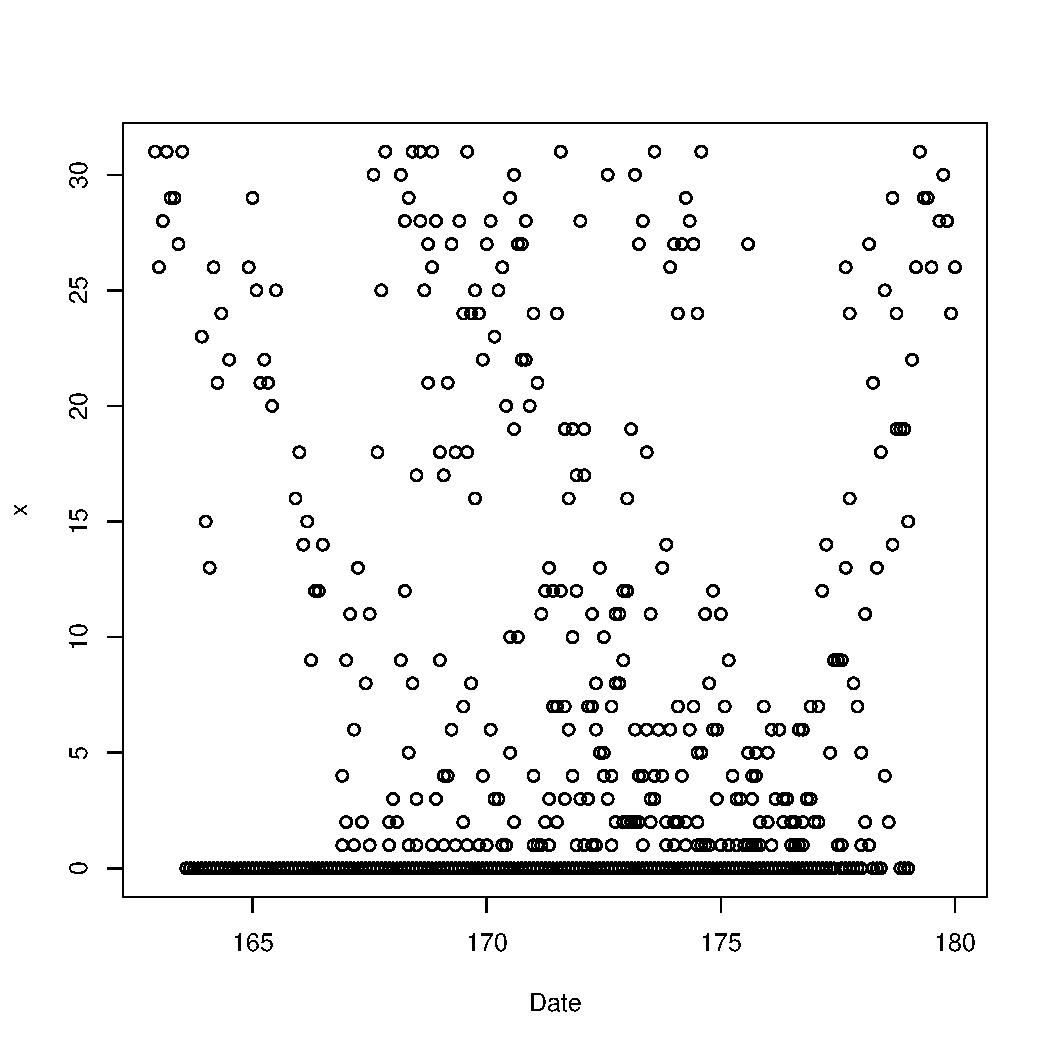
\includegraphics[width=\maxwidth]{figure/unnamed-chunk-19-1} 

\end{knitrout}

Third, we will need to decide what level of aggredation -- monthly, yearly, etc.  Let's aggreate by month and year to get monthly totals. 

There are loads of missing values in many months. Let's cut of the months that have more than 4 missing days. 

\begin{knitrout}
\definecolor{shadecolor}{rgb}{0.969, 0.969, 0.969}\color{fgcolor}\begin{kframe}
\begin{alltt}
\hlstd{TotalPPT} \hlkwb{<-} \hlkwd{aggregate}\hlstd{(Thailand}\hlopt{$}\hlstd{PRCP,} \hlkwd{list}\hlstd{(Thailand}\hlopt{$}\hlstd{Month, Thailand}\hlopt{$}\hlstd{Year), sum,} \hlkwc{na.rm}\hlstd{=T)}
\hlkwd{names}\hlstd{(TotalPPT)} \hlkwb{=} \hlkwd{c}\hlstd{(}\hlstr{"Group.1"}\hlstd{,} \hlstr{"Group.2"}\hlstd{,} \hlstr{"ppt"}\hlstd{)}
\hlstd{NonMissing} \hlkwb{<-} \hlstd{Missing[Missing}\hlopt{$}\hlstd{x} \hlopt{<} \hlnum{5}\hlstd{,} \hlkwd{c}\hlstd{(}\hlnum{1}\hlopt{:}\hlnum{3}\hlstd{)]}
\hlkwd{library}\hlstd{(dplyr)}
\end{alltt}


{\ttfamily\noindent\itshape\color{messagecolor}{\#\# \\\#\# Attaching package: 'dplyr'}}

{\ttfamily\noindent\itshape\color{messagecolor}{\#\# The following objects are masked from 'package:stats':\\\#\# \\\#\#\ \ \ \  filter, lag}}

{\ttfamily\noindent\itshape\color{messagecolor}{\#\# The following objects are masked from 'package:base':\\\#\# \\\#\#\ \ \ \  intersect, setdiff, setequal, union}}\begin{alltt}
\hlstd{PPT} \hlkwb{<-} \hlkwd{merge}\hlstd{(TotalPPT, NonMissing,} \hlkwc{all.y}\hlstd{=}\hlnum{TRUE}\hlstd{)}
\hlstd{PPT}\hlopt{$}\hlstd{Date} \hlkwb{<-} \hlkwd{as.numeric}\hlstd{(PPT}\hlopt{$}\hlstd{Group.1)} \hlopt{+} \hlkwd{as.numeric}\hlstd{(PPT}\hlopt{$}\hlstd{Group.2)}\hlopt{/}\hlnum{12}
\hlkwd{head}\hlstd{(PPT)}
\end{alltt}
\begin{verbatim}
##   Group.1 Group.2  ppt x     Date
## 1      01    1951  0.2 0 163.5833
## 2      01    1952  0.0 0 163.6667
## 3      01    1953 20.3 0 163.7500
## 4      01    1954  5.3 0 163.8333
## 5      01    1955  2.2 0 163.9167
## 6      01    1956  5.6 0 164.0000
\end{verbatim}
\end{kframe}
\end{knitrout}

First, we need a "mean" -- The IPCC uses 1961-1990 as a norm for temperature, I don't know what is the standard for rainfall or Thailand, so we should look that up. For now, we'll use our filtered records to generate a mean.

\begin{knitrout}
\definecolor{shadecolor}{rgb}{0.969, 0.969, 0.969}\color{fgcolor}\begin{kframe}
\begin{alltt}
\hlstd{PRCP_mean} \hlkwb{=} \hlkwd{mean}\hlstd{(PPT}\hlopt{$}\hlstd{ppt)}
\end{alltt}
\end{kframe}
\end{knitrout}

\begin{knitrout}
\definecolor{shadecolor}{rgb}{0.969, 0.969, 0.969}\color{fgcolor}\begin{kframe}
\begin{alltt}
\hlkwd{plot}\hlstd{(ppt}\hlopt{~}\hlstd{Date,} \hlkwc{data}\hlstd{=PPT)}
\hlkwd{abline}\hlstd{(}\hlkwc{h}\hlstd{=PRCP_mean,} \hlkwc{col}\hlstd{=}\hlstr{"blue"}\hlstd{)}
\end{alltt}
\end{kframe}
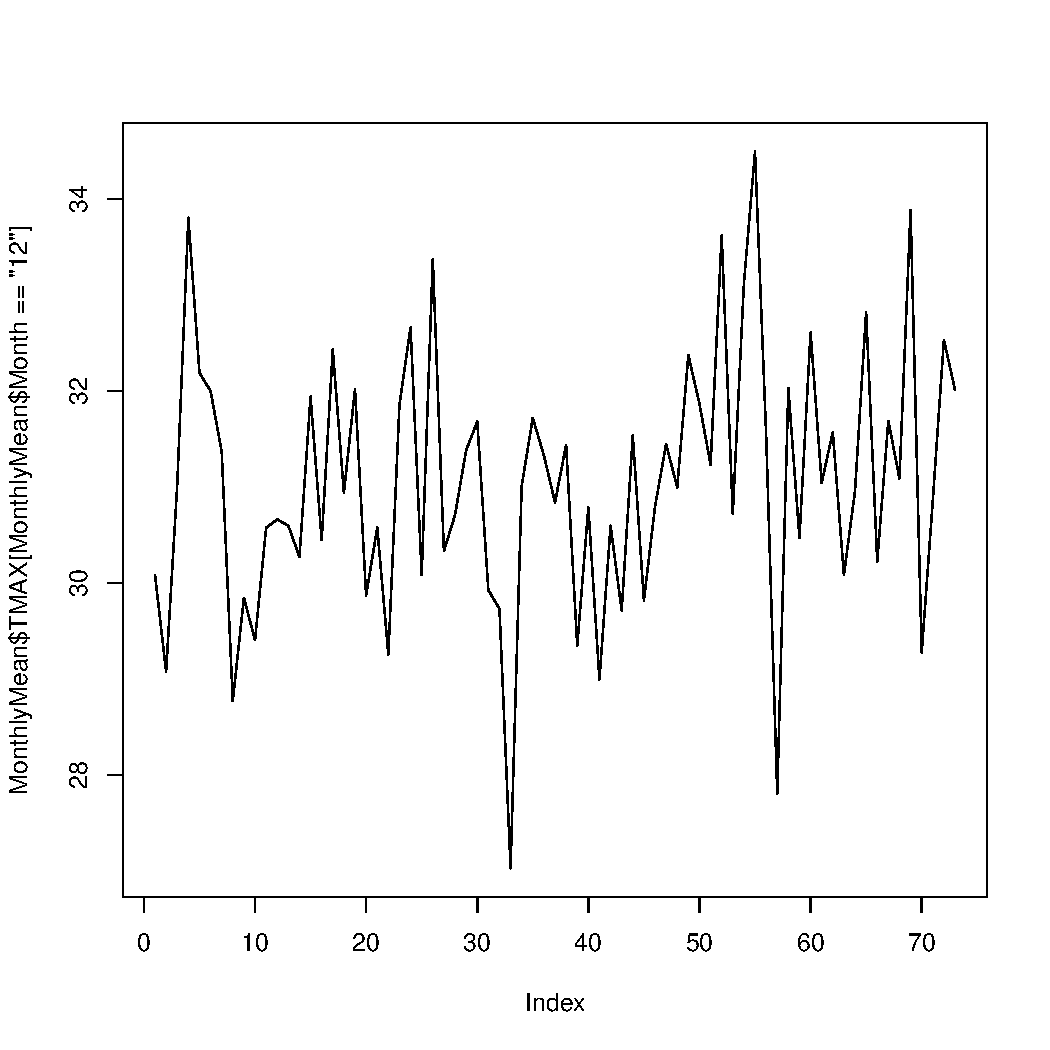
\includegraphics[width=\maxwidth]{figure/unnamed-chunk-22-1} 

\end{knitrout}

Wow, these data look terrible -- the mean looks meaningless given the biased data set. I don't think we can do more analysis with this. But let's look at a few months and see what we can decipher.

\begin{figure}
\begin{knitrout}
\definecolor{shadecolor}{rgb}{0.969, 0.969, 0.969}\color{fgcolor}
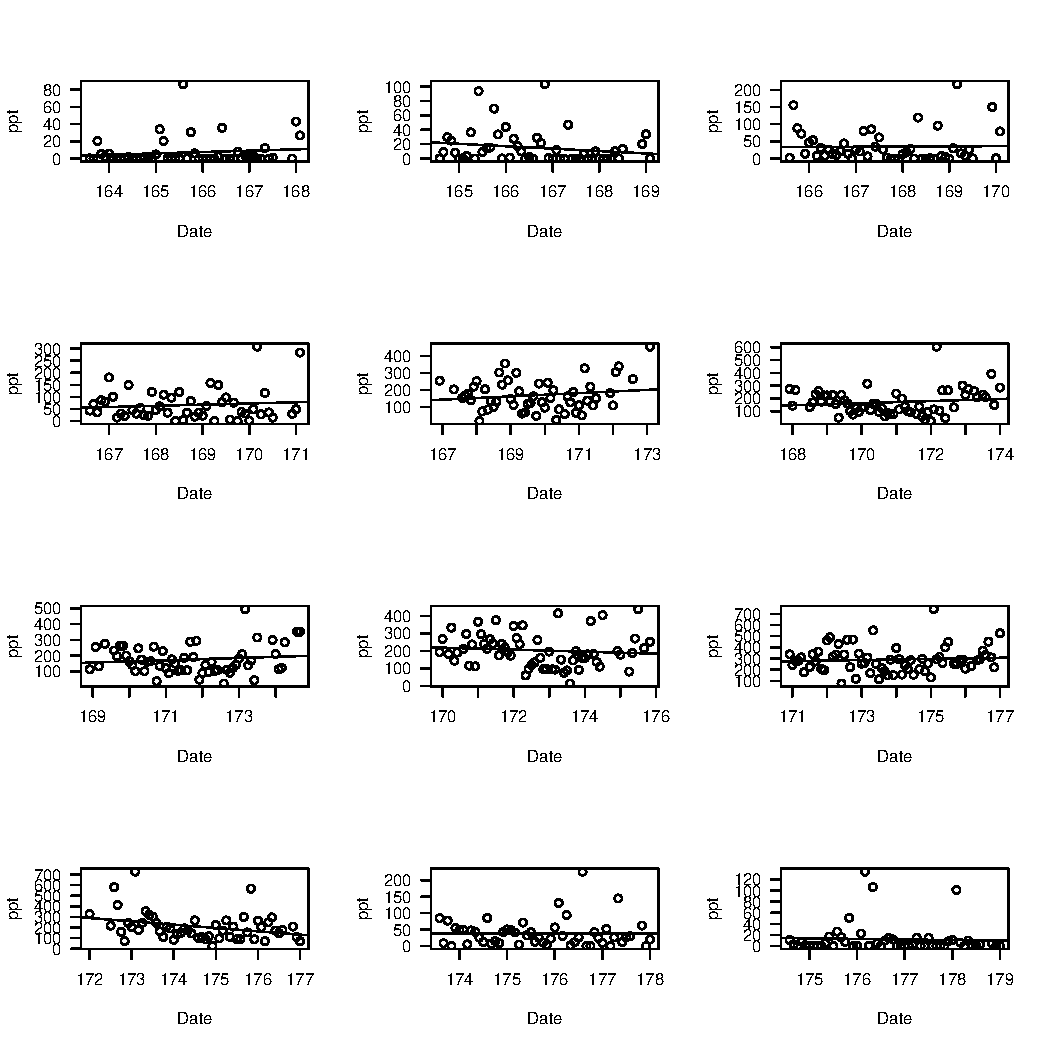
\includegraphics[width=\maxwidth]{figure/unnamed-chunk-23-1} 

\end{knitrout}
\end{figure}
 
%Fourth, in CA the water year starts in Oct 1. Should we follow the same convention?

\begin{knitrout}
\definecolor{shadecolor}{rgb}{0.969, 0.969, 0.969}\color{fgcolor}\begin{kframe}
\begin{alltt}
\hlcom{#LosAngeles$PRCP[LosAngeles$PRCP==-9999] <- NA}
\hlcom{#YearlySum = aggregate(PRCP ~ Year, LosAngeles, sum)}
\hlcom{#YearlySum$YEAR = as.numeric(YearlySum$Year) }
\hlcom{#YearlyMean = mean(YearlySum$PRCP)}
\end{alltt}
\end{kframe}
\end{knitrout}

A yearly mean, based on the annual sum for the entire records. Not sure this is appropriate.

Figure has points of the yearly sum of rainfall and the blue line mean. The greenline is the trend and red line is a five year running average, I think!  I am still trying to understand what the code is doing.

\begin{knitrout}
\definecolor{shadecolor}{rgb}{0.969, 0.969, 0.969}\color{fgcolor}\begin{kframe}
\begin{alltt}
\hlcom{#plot(PRCP~YEAR, data=YearlySum, las=1, ty="p")}
\hlcom{#abline(h=YearlyMean, col="blue")}
\hlcom{#YearlySum.lm = lm(PRCP~YEAR, data=YearlySum)}
\hlcom{#abline(coef(YearlySum.lm), col="green")}

\hlcom{#n <- 5}
\hlcom{#k <- rep(1/n, n)}
\hlcom{#k}

\hlcom{#y_lag <- stats::filter(YearlySum$PRCP, k, sides=1)}
\hlcom{#lines(YearlySum$YEAR, y_lag, col="red")}
\end{alltt}
\end{kframe}
\end{knitrout}

%The model suggests that the precipitation is declining at a rate of `r coef(YearlySum.lm)[2]` cm yr$^{-1}~$, or `r round(coef(YearlySum.lm)[2]*10, 2)` cm decade$^{-1}$.

\begin{knitrout}
\definecolor{shadecolor}{rgb}{0.969, 0.969, 0.969}\color{fgcolor}\begin{kframe}
\begin{alltt}
\hlcom{#summary(YearlySum.lm)}
\end{alltt}
\end{kframe}
\end{knitrout}

\subsection{Assumptions of the Linear Regression}

Regression models, like all statistics, rely on certain assumptions. Violations of these assumptions reduces the validity of the model. If the violations are serious, then the model could be misleading or even incorrect.

Here is a list of assumptions to produce a valid regression model:

\begin{description}
  \item[Homogeneity of Variance]
  \item[something else]
\end{description}

Assumptions about e , the “error term”: t
i. E(et
) = 0, zero mean
ii. E(et
) = s , constant variance 2 2
iii. E(et
, Xt
) = 0, no correlation with X 
iv. E(e , e ) , no autocorrelation. t t-1
v. e ~ Normally distributed (for hypothesis testing). t
3. Assumption four is especially important and most likely not to be met when
using time series data.

Autocorrelation.

1. It is not uncommon for errors to “track’ themselves; that is, for the error a time t to depend in part on its value at t - m, where m is a prior time period.

\subsubsection{Model Diagnostics}

With every statistical test done, researchers validate their model in some way or anther. Often this entails the use of diagnostics, a standardize battery of procedures to check to see if the data are following the assumptions. 

In R four plots are created by default.  To see them all at the same time, we need to change the graphical parameters so the graphics window expects four panels, in this case a 2 rows and two columns. 

\begin{knitrout}
\definecolor{shadecolor}{rgb}{0.969, 0.969, 0.969}\color{fgcolor}\begin{kframe}
\begin{alltt}
\hlkwd{par}\hlstd{(}\hlkwc{mfrow}\hlstd{=}\hlkwd{c}\hlstd{(}\hlnum{2}\hlstd{,}\hlnum{2}\hlstd{))}
\end{alltt}
\end{kframe}
\end{knitrout}

Try not to get bogged down in the code at this point. But it is a useful thing to remember.

% Additional LaTeX code to add caption to figure
\begin{figure}
\label{fig:diagnostics}
\caption{Default diagnostic plots for a linear model in R.}
%\setkeys{Gin}{width=0.75\textwidth} % LaTeX code to read the graphic file in at 75% of its original size
% R code chunk that produces a graphic
\begin{knitrout}
\definecolor{shadecolor}{rgb}{0.969, 0.969, 0.969}\color{fgcolor}\begin{kframe}
\begin{alltt}
\hlkwd{par}\hlstd{(}\hlkwc{mfrow}\hlstd{=}\hlkwd{c}\hlstd{(}\hlnum{2}\hlstd{,}\hlnum{2}\hlstd{))}
\hlkwd{plot}\hlstd{(}\hlkwd{lm}\hlstd{(TMAX} \hlopt{~} \hlstd{NewDate,} \hlkwc{data}\hlstd{=Thailand))}
\end{alltt}
\end{kframe}
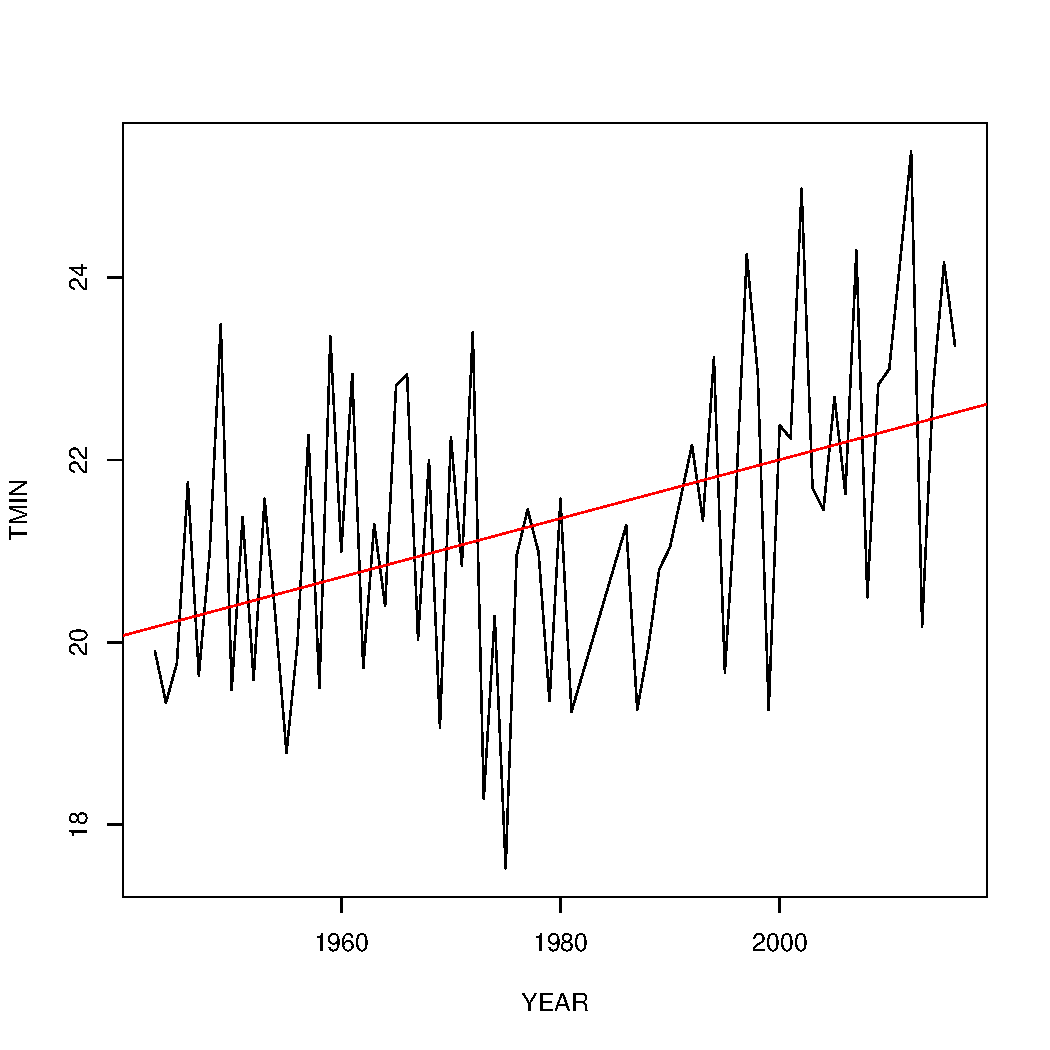
\includegraphics[width=\maxwidth]{figure/unnamed-chunk-28-1} 

\end{knitrout}
\end{figure}

To determine the validity of linear model assumptions (e.g. normality or heterogeneity of variance), you have probably used statistical tests; in contrast statisticians almost exclusively look at diagnostic plots. Why?  When assumptions are violated the tests to determine violations do not perform well. So, let's see how to look at these assumptions graphically with these diagnostic plots. Linear models should have diagnostic plots that do not have any obvious structure or pattern. In this case, Figure~\ref{fig:diagnostics} should show a great deal remaining structure in the residuals. Although for today, we are not going to try to interpret these figures, but you should notice there is a ton of unaccounted structure, i.e. variance, in the model. This is due, in part, to a violation of independence; these data are serially correlated and the model does not account for that and is inappropriate because of this. It also appears that a straight-line model does not fit well and a curvilinear should be investigated.

A properly specified model is shown in 

%Figure~\ref{fig:co2_data_mlo}. In this case, the trend line has been developing using a time series analysis, which is beyond the scope of this course. Nevertheless, you want to keep this in mind during the semester because we will see a fair amount of data that looks like this.

\section{The 'Null' Hypothesis versus Information Criteria}

\subsection{Model Comparison}

\subsection{AIC to make statements about strength of evidence}


\section{Relaxing Model Assumptions}

\subsection{Using Sources of Error in the Model}

Instead of letting autocorrelation be 'hidden' problem in the data, we can incorporate the correlation structure into the model and use it to our advantage -- create a better, i.e. unbiased estimate of the model parameters.

\subsection{Generalized Least Square (GLS) and Autocorrelation}

\begin{knitrout}
\definecolor{shadecolor}{rgb}{0.969, 0.969, 0.969}\color{fgcolor}\begin{kframe}
\begin{alltt}
\hlkwd{library}\hlstd{(nlme)}
\end{alltt}


{\ttfamily\noindent\itshape\color{messagecolor}{\#\# \\\#\# Attaching package: 'nlme'}}

{\ttfamily\noindent\itshape\color{messagecolor}{\#\# The following object is masked from 'package:dplyr':\\\#\# \\\#\#\ \ \ \  collapse}}\begin{alltt}
\hlcom{#TMAX.gls = gls(TMAX ~ NewDate, data = Thailand, na.action=na.omit)}
\hlcom{#summary(TMAX.gls)}
\hlcom{#TMAX.gls2 = gls(TMAX ~ NewDate, data = Thailand, correlation = corAR1(form=~1), na.action=na.omit)}
\hlcom{#summary(TMAX.gls2)}

\hlcom{#anova(TMAX.gls, TMAX.gls2)}
\end{alltt}
\end{kframe}
\end{knitrout}


\subsection{Adding Seasonality}


\section{More Sophisticated Approaches}

\section{Advanced Methods}

You may want to examine the GAM package in R, as it can be adapted to do some (or all) of what you are looking for. The original paper (Hastie \& Tibshirani, 1986) is available via OpenAccess if you're up for reading it.

Essentially, you model a single dependent variable as being an additive combination of 'smooth' predictors. One of the typical uses is to have time series and lags thereof as your predictors, smooth these inputs, then apply GAM.

This method has been used extensively to estimate daily mortality as a function of smoothed environmental time series, especially pollutants. It's not OpenAccess, but (Dominici et al., 2000) is a superb reference, and (Statistical Methods for Environmental Epidemiology with R) is an excellent book on how to use R to do this type of analysis.

\section{Time Series Analysis}

Time series analysis

Time series analysis refers to a particular collection of specialised regression methods that use integrated moving averages and other smoothing techniques to illustrate trends in the data. It involves a complex process that incorporates information from past observations and past errors in those observations into the estimation of predicted values.

Moving averages provide a useful way of presenting time series data, highlighting any long-term trends whilst smoothing out any short-term fluctuations. They are also commonly used to analyse trends in financial analysis. The calculation of moving averages is described in more detail here.

Methods for time series analyses may be divided into two classes: frequency-domain methods and time-domain methods. The former include spectral analysis and recently wavelet analysis; the latter include auto-correlation and cross-correlation analysis. In time domain correlation analyses can be made in a filter-like manner using scaled correlation, thereby mitigating the need to operate in frequency domain.

Whether or not you wish to forecast or not has nothing whatsoever to do with correct time series analysis. Time series methods can develop a robust model which can be used simply to characterize the relationship between a dependent series and a set of user-suggested inputs (a.k.a. user-specified predictor series) and empirically identified omitted variables be they deterministic or stochastic.Users at their option can then extend the "signal" into the future i.e. forecast with uncertainties based upon the uncertainty in the coefficients and the uncertainty in the future values of the predictor . Now these two kinds of empirically identified "omitted series" can be classified as 1) deterministic and 2) stochastic. The first type are simply Pulses, Level Shifts , Seasonal Pulses and Local Time Trends whereas the second type is represented by the ARIMA portion of your final model. When one omits one or more stochastic series from the list of possible predictors, the omission is characterized by the ARIMA component in your final model. Time series modelers refer to ARIMA models as a "Poor Man's Regression Model" because the past of the series is being used as a proxy for omitted stochastic input series.

\section{References}

%Bailey L, Vardulaki K, Langham J, Chandramohan D. Introduction to Epidemiology. Open University Press, 2005.

%www.mchb.hrsa.gov/mchirc/_pubs/trend_analysis.pdf

\end{document}
